% Preamble
\documentclass{article}

% Packages
\usepackage{docmute} % LaTeX 合并独立子文件
\usepackage{amsmath} % Advanced math typesetting
\usepackage[utf8]{inputenc} % Unicode support (Umlauts etc.)
\usepackage[ngerman]{babel} % Change hyphenation rules
\usepackage{hyperref} % Add a link to your document
\usepackage{graphicx} % Add pictures to your document
\usepackage{subcaption}
% \usepackage{graphicspath} % Add pictures in folder to your document
\usepackage{listings} % Source code formatting and highlighting
\usepackage{booktabs}
\usepackage{xcolor} % add color to text
\usepackage{color}
\usepackage[backend=biber]{biblatex}
\usepackage{siunitx} % Required for alignment
\usepackage{enumitem} % enumerate can use other order symbol
\usepackage{multirow} % Required for multirows
\usepackage{longtable} % To display tables on several pages
\usepackage{rotating} % To display tables in landscape
% \usepackage{booktabs} % For \toprule, \midrule and \bottomrule
% \usepackage{siunitx} % Formats the units and values
\usepackage{pgfplotstable} % Generates table from .csv
% \usepackage{siunitx}
\usepackage{tikz} % To generate the plot from csv
\usepackage{pgfplots}
\usepackage{tikz}
\usepackage{circuitikz}

\pgfplotsset{compat=newest} % Allows to place the legend below plot
\usepgfplotslibrary{units} % Allows to enter the units nicely
\addbibresource{ref.bib} % add references
% \graphicspath{{graphics/}} % graphicspath's images path

% Main document
\begin{document} % Set up the maketitle command
\author{Massyao Tse}
\title{Learning \LaTeX{}}
\date{\today{}} % You can remove \today{} and type a date manually


\maketitle{} % Generates title
\newpage

\tableofcontents{} % Generates table of contents from sections

% How to use LaTeX
% --------------------------------
% -------  chapter 1  ------------
% --------------------------------
\maketitle
\newpage
\section{How to use \LaTeX{}}
This is a quick introduction to the most common features of \LaTeX{}. For more features, check the other lessons on \url{http://www.latex-tutorial.com} and the articles on \url{http://blog.latex-tutorial.com}. 
\subsection{Document structure}
The documents in \LaTeX{} are structured slightly different from Word. The document consists of two parts, the preamble and the main document. If you're familiar with programming, then you might want to compare the structure with that of a C/C++ file.

\subsubsection{Preamble}
The purpose of the preamble is to tell \LaTeX{} what kind of document you will set up and what packages you are going to need. A package is a set of additional functions such as \emph{amsmath} for additional math formatting. For this document, the preamble looks like this:

\begin{lstlisting}[language={[LaTeX]TeX},caption=Preamble of this document,breaklines=true,frame=single]
% Preamble
% ---
\documentclass{article}

% Packages
% ---
\usepackage{amsmath} % Advanced math typesetting
\usepackage[utf8]{inputenc} % Unicode support (Umlauts etc.)
\usepackage[ngerman]{babel} % Change hyphenation rules
\usepackage{hyperref} % Add a link to your document
\usepackage{graphicx} % Add pictures to your document
\usepackage{listings} % Source code formatting and highlighting
\end{lstlisting}

You can set the class of the documentclass with the \emph{documentclass} command and add packages with the \emph{usepackage} command. Only the \emph{documentclass} command is mandatory, you can compile a document also without packages, yet some functions may be missing in this case. The \emph{usepackage} command \emph{must not} be used in the main document.

\subsubsection{Main document}
The main document is contained within the \emph{document} environment like this:

\begin{lstlisting}[language={[LaTeX]TeX},caption=Main part of a \LaTeX{} document.,breaklines=true,frame=single,frame=single]
\begin{document}
% ...
% ... Text goes here
% ...
\end{document}
\end{lstlisting}

Within those two statements, we can add the content of our document. But just adding the text is probably not enough, since we also have to apply formatting to it.

\subsection{Formatting in \LaTeX{}}
Formatting in \LaTeX{} can be applied by the use of commands and environment. The topmost environment is the document environment as described in Listing ref{lst:main}. So there are obviously more environments, but how to find them? Well the easiest way is to download a \LaTeX{} cheat sheet which provides a list of the most useful commands and environments. For most packages there is also a manual available, which can be found on Google.

\subsubsection{Math typesetting}
To introduce you to math typesetting and environments, I will demonstrate you how to format some simple equations:

\begin{align}
f(x) &= x^2\\
f'(x) &= 2x\\
F(x) &= \int^a_b f(x)dx\\
F(x) &= \frac{1}{3}x^3\\
M(A) &= \left[
    \begin{matrix}
    f(x) & g(x)\\
    f'(x) & g'(x)
    \end{matrix}
    \right]\\
H(f) &= \int\left\{\frac{\lambda}{\sqrt{x}}\right\}^3dx
\end{align}



This can be done with the following code:

\begin{lstlisting}[language={[LaTeX]TeX},caption=Typesetting equations in \LaTeX{}.,breaklines=true,frame=single]
\begin{align}
f(x) &= x^2\\
f'(x) &= 2x\\
F(x) &= \int f(x)dx\\
F(x) &= \frac{1}{3}x^3
\end{align}
\end{lstlisting}

As you can see, we again have a \emph{begin} and \emph{end} statement, this it's applying the \emph{align} environment. This will align the equations at the ampersand (\&) sign. Naturally, those will be placed in front of the equality sign. If you watched carefully, you will see that \LaTeX{} magically added sequential numbers to all equations. \LaTeX{} does this for many other elements too. More about that in the next chapter.

\subsubsection{Document layout}
Usually a document does not only consist of a bunch of equations, but needs some kind of structure too. We are usually going to need at least:

\begin{itemize}
\item{Title/Titlepage}
\item{Table of contents}
\item{Headlines/Sections}
\item{Bibliography}
\end{itemize}

\LaTeX{} provides all the commands we need. The following commands will help us:\\

\begin{lstlisting}[language={[LaTeX]TeX},caption=Useful commands to structure a document.,label=lst:main,breaklines=true,frame=single]
\section{Text goes here} % On top of document hierarchy; automatically numbered
\subsection{}
\subsubsection{}
\paragraph{} % Paragraphs have no numbering
\subparagraph{}

\author{Claudio Vellage} % The authors name
\title{A quick start to \LaTeX{}} % The title of the document
\date{\today{}} % Sets date you can remove \today{} and type a date manually
\maketitle{} % Generates title
\tableofcontents{} % Generates table of contents from sections and subsections

\\ % Linebreak
\newpage{} % Pagebreak
\end{lstlisting}

There are commands to create sections, the sections are numbered automatically and the \emph{tableofcontents} command will use them to generate the table of contents. You don't have to do it yourself, ever. \LaTeX{} also provides commands to generate the title using the \emph{maketitle} command. This needs the \emph{author}, \emph{title} and \emph{date} command to be set. If you place the \emph{maketitle} or \emph{tableofcontents} command in your document, the Commands will be added at that exact place, so you probably want them in the very beginning of your document. If you want the title to appear on a single page, simply use the \emph{newline} command.

\subsubsection{Adding a picture}

Most documents will also need some kind of picture. Like this:

\begin{figure}
\includegraphics[width=1.0\textwidth]{picture}
\caption{This figure shows the logo of my website.}
\end{figure}

 Adding them is fairly easy:

\begin{lstlisting}[language={[LaTeX]TeX},caption=Adding pictures in \LaTeX{}.,breaklines=true,frame=single]
\begin{figure}
\includegraphics[width=\textwidth]{picture.png}
\caption{This figure shows the logo of my website.}
\end{figure}
\end{lstlisting}

You have to embed the picture within the \emph{figure} environment, then use the \emph{includegraphics} command to select the image. Note that the picture file has to be in the same directory as your .tex file or you specify the path like this:
\begin{lstlisting}[language={[LaTeX]TeX},caption=How to specify a path.,breaklines=true,frame=single]
% ...
\includegraphics[width=\textwidth]{FOLDERNAME/picture.png}
% ...
\end{lstlisting}

It makes sense to manage all your pictures in subfolders if you have many of them.

\subsection{Sourcecode formatting}

Throughout the book I used the \emph{listings} package to format the \LaTeX{} code snippets. You can specify the language for each \emph{lstlistings} block, in this case i used \LaTeX{} of course and added a caption as well as enabled linebreaking:

\begin{lstlisting}[language={[LaTeX]TeX},caption=How to use the listings package.",breaklines=true,frame=single,escapechar=^]
^\textbackslash^begin{lstlisting}[language={[LaTeX]TeX},caption=,breaklines=true,frame=single]
% Source code goes here
^\textbackslash^end{lstlisting}
\end{lstlisting}

The language is specified as \emph{[DIALECT]LANGUAGE}, here \LaTeX{} is dialect of \TeX{}. A list of all programming languages can be obtained from the \emph{listings} package manual, but you can also just try out if it works.

%\subsubsection{References and Bibliography}\label{sec:ref}
\subsubsection{References and Bibliography}
%You can specify labels for all the things that are automatically numbered. If you want to refer to a section of your document, you'd simply use the \emph{label} and \emph{ref} (reference) command. Where the label indicates what you want to refer to and the reference will print the actual number of the element in your document. This will also work interactively in your PDF reader You can try this feature in section \ref{sec:ref}.

\begin{lstlisting}[language={[LaTeX]TeX},caption=Labels and references in \LaTeX{},breaklines=true,frame=single]
\section{}\label{sec:YOURLABEL}
% ...
I've written text in section \ref{sec:YOURLABEL}.
\end{lstlisting}

Papers usually include a lot of references to the great works of other people. In order to properly cite them, we'd want to use the biblatex package. For this purpose we'd simply add the following code to our preamble:

\begin{lstlisting}[language={[LaTeX]TeX},caption=Preamble code to use biblatex.,breaklines=true,frame=single]
\usepackage[backend=bibtex,style=verbose-trad2]{biblatex} % Use biblatex package
\bibliography{FILENAME} % The name of the .bib file (name without .bib)
\end{lstlisting}

All bibliographic information will be stored in the bibliography (.bib) and \emph{must not} be inside of the .tex file An example could look like this:

\begin{lstlisting}[language={[LaTeX]TeX},caption=Example bibliography file.,breaklines=true,frame=single]
@ARTICLE=
{
VELLAGE:1,
AUTHOR="Claudio Vellage",
TITLE="A quick start to \LaTeX{}",
YEAR="2013",
PUBLISHER="",
}
\end{lstlisting}

Now i could add a self reference using the \emph{cite} command:

\begin{lstlisting}[language={[LaTeX]TeX},caption=The cite command.,breaklines=true,frame=single]
This feature works as I described in \cite{VELLAGE:1}.
\end{lstlisting}

The \emph{biblatex} is very smart and wil print autogenerate the bibliography if we want to. We'd usually do this in the end of the document. Simply add

\begin{lstlisting}[language={[LaTeX]TeX},caption=The cite command.,breaklines=true,frame=single]
\printbibliography
\end{lstlisting}

to our document. More examples can be found on the \href{http://www.latex-tutorial.com/lesson7/}{website}.

\subsubsection{Code}

  \lstdefinestyle{lfonts}{
    basicstyle   = \footnotesize\ttfamily,
    stringstyle  = \color{purple},
    keywordstyle = \color{blue!60!black}\bfseries,
    commentstyle = \color{olive}\scshape,
  }
  \lstdefinestyle{lnumbers}{
    numbers     = left,
    numberstyle = \tiny,
    numbersep   = 1em,
    firstnumber = 1,
    stepnumber  = 1,
  }
  \lstdefinestyle{llayout}{
    breaklines       = true,
    tabsize          = 2,
    columns          = flexible,
  }
  \lstdefinestyle{lgeometry}{
    xleftmargin      = 20pt,
    xrightmargin     = 0pt,
    frame            = tb,
    framesep         = \fboxsep,
    framexleftmargin = 20pt,
  }
  \lstdefinestyle{lgeneral}{
    style = lfonts,
    style = lnumbers,
    style = llayout,
    style = lgeometry,
  }
  \lstdefinestyle{python}{
      language = {Python},
      style    = lgeneral,
  }

  \lstinline[style = python]|print('Hello world!')|
  \begin{lstlisting}[style = python]
  for x in range(101):
      print('fizz'[x%3*4:] + 'buzz'[x%5*4:] or x)
  \end{lstlisting} 


\begin{lstlisting}[language={[LaTeX]TeX},caption=code in \LaTeX{},breaklines=true,frame=single]
  \documentclass{article}
  \usepackage{xcolor}
  \usepackage{listings}
  \lstdefinestyle{lfonts}{
    basicstyle   = \footnotesize\ttfamily,
    stringstyle  = \color{purple},
    keywordstyle = \color{blue!60!black}\bfseries,
    commentstyle = \color{olive}\scshape,
  }
  \lstdefinestyle{lnumbers}{
    numbers     = left,
    numberstyle = \tiny,
    numbersep   = 1em,
    firstnumber = 1,
    stepnumber  = 1,
  }
  \lstdefinestyle{llayout}{
    breaklines       = true,
    tabsize          = 2,
    columns          = flexible,
  }
  \lstdefinestyle{lgeometry}{
    xleftmargin      = 20pt,
    xrightmargin     = 0pt,
    frame            = tb,
    framesep         = \fboxsep,
    framexleftmargin = 20pt,
  }
  \lstdefinestyle{lgeneral}{
    style = lfonts,
    style = lnumbers,
    style = llayout,
    style = lgeometry,
  }
  \lstdefinestyle{python}{
      language = {Python},
      style    = lgeneral,
  }
  \begin{document}
  \lstinline[style = python]|print('Hello world!')|
  \begin{lstlisting}[style = python]
  for x in range(101):
      print('fizz'[x%3*4:] + 'buzz'[x%5*4:] or x)
  \end\{lstlisting\} 
  \end{document}
  \end{lstlisting}
  

% LaTeX Math Symbols - A glossary
% --------------------------------
% -------  chapter 2  ------------
% --------------------------------
\maketitle
\newpage

\section{LaTeX Math Symbols - A glossary}
An overview of commonly used math symbols in LaTeX with a sandbox to try them out immediately in your browser.

Since LaTeX offers a large amount of features, it's hard to remember all commands. Even though commands follow a logical naming scheme, you will probably need a table for the most common math symbols at some point. You can play around with the commands shown here in the sandbox below and insert your equation into your LaTeX document. I don't want to provide a complete list of LaTeX symbols on this website. The ctan alreadyprovides a huge list with currently 5913 symbols, which you can download here. Instead I'm trying to limit this list to the most common math symbols and commands. If you think I forgot some very important basic function or symbol here, please let me know.

\subsection{List of common LATEX math symbols}
Trigonometric functions
Integrals
Matrices
Dots
Miscellaneous functions
Sandbox




\subsubsection{Trigonometric functions}
The symbols for trigonometric functions have a very straightforward naming scheme. Just precede the common abbreviations with a backslash \textbackslash and put your variables in braces.

\begin{center}
\begin{tabular}{ccc}
\toprule  %添加表格头部粗线
Name &	Symbol &	Command\\
\midrule  %添加表格中横线
Sine &  $\sin x$ & \textbackslash sin x \\
Cosine &  $\cos x$ & \textbackslash cos x \\
Tangent &  $\tan x$ & \textbackslash tan x \\
Cotangent &  $\cot x$ & \textbackslash cot x\\
Secant &  $\sec x$ & \textbackslash sec x \\
Cosecant &  $\csc x$ & \textbackslash csc x\\
\bottomrule %添加表格底部粗线
\end{tabular}
\end{center}




\subsubsection{Integrals}
LaTeX offers math symbols for various kinds of integrals out of the box.
Note that you can set the integral boundaries by using the underscore \_ and 
circumflex \^ symbol as seen below.

\begin{center}
\begin{tabular}{ccc}
\toprule  %添加表格头部粗线
Name&	Symbol&	Command\\
\midrule  %添加表格中横线
Indefinite integral & $\int f(x) dx$ & \textbackslash int f(x) dx \\
Definite integral & $\int_a^b f(x) x$ & \textbackslash int\_{} a\^{} b f(x) x \\
Domain integral &  $\int_D f(x) dx$ & \textbackslash int\_{} D f(x) dx \\
Double integral & $\iint f(x,y) dx dy$ & \textbackslash iint f(x,y) dx dy \\
Triple integral & $\iiint f(x,y,z) dx dy dz$ & \textbackslash iiint f(x,y,z) dx dy dz \\
Closed curve integral & $\oint_C F ds$ & \textbackslash oint\_{} C F ds \\
\bottomrule %添加表格底部粗线
\end{tabular}
\end{center}



\subsubsection{Matrices}
Of course LaTeX is able to typeset matrices as well. 
For this purpose LaTeX offers the following environments. 
Columns are separated with ampersand \& and rows with a double backslash \textbackslash\textbackslash (the linebreak command). Make sure that the number of ampersands is the same for every row.

\begin{center}
\begin{tabular}{ccc}
\toprule  %添加表格头部粗线
Name&	Symbol&	Command\\
\midrule  %添加表格中横线
Matrix 
  & $\begin{matrix}1&0\\1&0\end{matrix}$ 
  & \textbackslash begin\textbackslash\{matrix\}1\&0 \textbackslash\textbackslash 1\&0\textbackslash end\{matrix\} \\
\\
bMatrix 
  & $\begin{bmatrix}1&0\\1&0\end{bmatrix}$ 
  & \textbackslash begin\textbackslash\{bmatrix\}1\&0 \textbackslash\textbackslash 1\&0\textbackslash end\{bmatrix\} \\
\\
pMatrix 
  & $\begin{pmatrix}1&0\\1&0\end{pmatrix}$ 
  & \textbackslash begin\textbackslash\{pmatrix\}1\&0 \textbackslash\textbackslash 1\&0\textbackslash end\{pmatrix\} \\
\\
vMatrix 
  & $\begin{vmatrix}1&0\\1&0\end{vmatrix}$ 
  & \textbackslash begin\textbackslash\{vmatrix\}1\&0 \textbackslash\textbackslash 1\&0\textbackslash end\{vmatrix\} \\
\\
Determinant 
  & $\det{\begin{vmatrix}1&0\\1&0\end{vmatrix}}$ 
  & \textbackslash det\{\textbackslash begin\{vmatrix\}1\&0 \textbackslash\textbackslash 1\&0\textbackslash end\{vmatrix\}\} \\
\bottomrule %添加表格底部粗线
\end{tabular}
\end{center}
If you want to typeset very large matrices, the following commands can become in handy as well.




\subsubsection{Dots}
The most common dot symbols used in math notation are available in LaTeX as well.

\begin{center}
\begin{tabular}{ccc}
\toprule  %添加表格头部粗线
Name&	Symbol&	Command\\
\midrule  %添加表格中横线
Middot \/ Centered dot
  & $\cdot$
  & \textbackslash cdot\\
\\
Horizontal Dots \/ Centered dots 
  & $\cdots$
  & \textbackslash cdots\\
\\
Vertical Dots 
  & $\vdots$
  & \textbackslash vdots\\
\\
Diagonal Dots 
  & $\ddots$
  & \textbackslash ddots\\
\\
Lower Dots 
  & $\ldots$
  & \textbackslash ldots\\
\bottomrule %添加表格底部粗线
\end{tabular}
\end{center}

matrix     
$\begin{bmatrix}
  1 & 0 & \cdots & 0\\
  1 & 0 & \cdots & 0\\
  \vdots & \vdots & \ddots & \vdots \\
  1 & 0 & 0 & 0
  \end{bmatrix}$, 
  \\
  code will be ,\\
  \textbackslash begin\{bmatrix\}
  1 \& 0 \& \textbackslash cdots \& 0 \textbackslash\textbackslash
  1 \& 0 \& \textbackslash cdots \& 0\textbackslash\textbackslash
  \textbackslash vdots \& \textbackslash vdots \& \textbackslash ddots \& \textbackslash vdots \textbackslash\textbackslash
  1 \& 0 \& 0 \& 0
  \textbackslash end\{bmatrix\}



  \subsubsection{Matrices}
  Of course LaTeX is able to typeset matrices as well. 
  For this purpose LaTeX offers the following environments. 
  Columns are separated with ampersand \& and rows with a double backslash \textbackslash\textbackslash (the linebreak command). Make sure that the number of ampersands is the same for every row.
  
  \begin{center}
  \begin{tabular}{ccc}
  \toprule  %添加表格头部粗线
  Name&	Symbol&	Command\\
  \midrule  %添加表格中横线
  Matrix 
    & $\begin{matrix}1&0\\1&0\end{matrix}$ 
    & \textbackslash begin\textbackslash\{matrix\}1\&0 \textbackslash\textbackslash 1\&0\textbackslash end\{matrix\} \\
  \\
  bMatrix 
    & $\begin{bmatrix}1&0\\1&0\end{bmatrix}$ 
    & \textbackslash begin\textbackslash\{bmatrix\}1\&0 \textbackslash\textbackslash 1\&0\textbackslash end\{bmatrix\} \\
  \\
  pMatrix 
    & $\begin{pmatrix}1&0\\1&0\end{pmatrix}$ 
    & \textbackslash begin\textbackslash\{pmatrix\}1\&0 \textbackslash\textbackslash 1\&0\textbackslash end\{pmatrix\} \\
  \\
  vMatrix 
    & $\begin{vmatrix}1&0\\1&0\end{vmatrix}$ 
    & \textbackslash begin\textbackslash\{vmatrix\}1\&0 \textbackslash\textbackslash 1\&0\textbackslash end\{vmatrix\} \\
  \\
  Determinant 
    & $\det{\begin{vmatrix}1&0\\1&0\end{vmatrix}}$ 
    & \textbackslash det\{\textbackslash begin\{vmatrix\}1\&0 \textbackslash\textbackslash 1\&0\textbackslash end\{vmatrix\}\} \\
  \bottomrule %添加表格底部粗线
  \end{tabular}
  \end{center}
  If you want to typeset very large matrices, the following commands can become in handy as well.
  
  
  
  
  \subsubsection{Miscellaneous Functions}
  Here are some more basic functions which don't fit in the categories mentioned above.
  \begin{center}
  \begin{tabular}{ccc}
  \toprule  %添加表格头部粗线
  Name&	Symbol&	Command\\
  \midrule  %添加表格中横线
  Logarithmic Function / Logarithm
    & $\log{x}$
    & \textbackslash log\{x\}\\
  \\
  Logarithm (base a)
    & $\log_a{b}$
    & \textbackslash log\_a\{b\}\\
  \\
  Square root function / Square root
    & $\sqrt{x}$
    & \textbackslash sqrt\{x\}\\
  \\
  n-th root function / n-th root
    & $\sqrt[n]{x}$
    & \textbackslash sqrt[n]\{x\}\\
  \\
  Rational function / Fraction
    & $\frac{u(x)}{v(x)}$
    & \textbackslash frac\{u(x)\}\{v(x)\}\\
  \bottomrule %添加表格底部粗线
  \end{tabular}
  \end{center}
  
  
  \subsection{Greek alphabet}
  Learn the LaTeX commands to display the greek alphabet. A rendered preview of all letters is shown alongside all commands in a nice table.
  \begin{center}
  \begin{tabular}{ccc}
  \toprule  %添加表格头部粗线
  Name&	Symbol&	Command\\
  \midrule  %添加表格中横线
  Alpha	 & $\alpha A$ & \textbackslash alpha A \\
  Beta	 & $\beta B$ & \textbackslash beta B \\
  Gamma	 & $\gamma \Gamma $ & \textbackslash gamma \textbackslash Gamma\\
  Delta	 & $\delta  \Delta $ & \textbackslash delta  \textbackslash Delta\\
  Zeta	 & $\zeta  Z$ & \textbackslash zeta  Z \\
  Eta	 & $\eta E$ & \textbackslash eta E \\
  Theta	 & $\theta \Theta$ & \textbackslash theta \textbackslash Theta \\
  Iota	 & $\iota I$ & \textbackslash iota I \\
  Kappa	 & $\kappa K$ & \textbackslash kappa K \\
  Lambda	 & $\lambda \Lambda$ & \textbackslash lambda \textbackslash Lambda \\
  Mu	 & $\mu M$ & \textbackslash mu M \\
  Nu	 & $\nu N$ & \textbackslash nu N \\
  % Omicron	 & $\omicron O$ & \textbackslash omicron O \\
  Pi	 & $\pi \Pi$ & \textbackslash pi \textbackslash Pi \\
  Rho	 & $\rho R$ & \textbackslash rho R \\
  Sigma	 & $\sigma \Sigma$ & \textbackslash sigma \textbackslash Sigma \\
  Tau	 & $\tau T$ & \textbackslash tau T \\
  Upsilon	 & $\upsilon \Upsilon$ & \textbackslash upsilon \textbackslash Upsilon \\
  Phi	 & $\phi \Phi$ & \textbackslash phi \textbackslash Phi\\
  Chi	 & $\chi X$ & \textbackslash chi X \\
  Psi	 & $\psi \Psi$ & \textbackslash psi \textbackslash Psi \\
  Omega	 & $\omega \Omega$ & \textbackslash omega \textbackslash Omega \\
  \bottomrule %添加表格底部粗线
  \end{tabular}
  \end{center}

  \subsection{Text Formatting}
    This website provides an overview of basic text
    formatting commands in LaTeX. Most commands are 
    very straightforward to use. I personally think
    there will be few usecases to manually adjust 
    the settings of the font, because the environments 
    usually do this job for you automatically, 
    I just included this for completeness.
  \subsubsection{Font Size}
  \begin{center}
  \begin{tabular}{ccc}
  \toprule  %添加表格头部粗线
  Name&	Symbol&	Command\\
  \midrule  %添加表格中横线
    Tiny & $ {\tiny Text} $ & \{\textbackslash tiny Text\} \\
    Small & $ {\small Text} $ & \{\textbackslash small Text\} \\
    Normal & $ {\normalsize Text} $ & \{\textbackslash normalsize Text\} \\
    Large & $ {\large Text} $ & \{\textbackslash large Text\} \\
    Huge & $ {\huge Text} $ & \{\textbackslash huge Text\} \\
  \bottomrule %添加表格底部粗线
  \end{tabular}
  \end{center}
  \subsubsection{Font Style}
  \begin{center}
  \begin{tabular}{ccc}
  \toprule  %添加表格头部粗线
  Name&	Symbol&	Command\\
  \midrule  %添加表格中横线
    Bold & $ \textbf{Text} $ & \textbackslash textbf\{Text\} \\
    Italic & $ \textit{Text} $ & \textbackslash textit\{Text\} \\
    Typewriter & $ \texttt{Text} $ & \textbackslash texttt\{Text\} \\
    % Sans-Serif & $ \ltexts{fText} $ & \textbackslash ltexts\{fText\} \\
    Serif (Roman) & $ \textrm{Text} $ & \textbackslash textrm\{Text\} \\
    Underline & $ \underline{Text} $ & \textbackslash underline\{Text\} \\
  \bottomrule %添加表格底部粗线
  \end{tabular}
  \end{center}

  %  js code to convert code to latex text
  % const str_replace = str =>{
  %   return str.replace(/\\/g, '\\textbackslash ')
  %             .replace(/{/g, '\\{')
  %             .replace(/}/g, '\\}')
  %             .replace('&nbsp;', ' ')
  % }
  % $$('tr').map(tr_ele => {
  %   const str1 = tr_ele.childNodes[0].innerHTML
  %   const str2 = tr_ele.childNodes[2].innerHTML.replace('&nbsp;', ' ')
  %   const str3 = str_replace(tr_ele.childNodes[2].innerHTML)
  %   console.log(str1,str2,str3)
  %   const str = `${str1} & $ ${str2} $ & ${str3} \\\\`
  %   return str
  % }).join('\n')

% Figure or Picture
% --------------------------------
% -------  chapter 3  ------------
% --------------------------------
\maketitle
\newpage

\section{Figure or Picture}
  \textbf{Learn how to insert images and caption them. 
    Examples for a single figure, and multiple figures 
    next to each other, using the subfigure environment.}
  \subsection{Captioned images / figures in LaTeX}
    From time to time, it's necessary to add pictures
    to your documents. Using LaTeX all pictures will 
    be indexed automatically and tagged with successive
    numbers when using the \textit{figure environment} 
    and the graphicx package.


    %  lstlisting verbatim minted
    \begin{lstlisting}[language={[LaTeX]TeX}, breaklines=true,frame=single]
      % \begin{verbatim}
        \documentclass{article}
    
        \usepackage{graphicx}
        
        \begin{document}
        
        \begin{figure}
          \includegraphics[width=\linewidth]{boat.jpg}
          \caption{A boat.}
          \label{fig:boat1}
        \end{figure}
        
        Figure \ref{fig:boat1} shows a boat.
        \end{document}
      % \end{verbatim}
    \end{lstlisting}

    \begin{figure}[h!]
      \includegraphics[width=\linewidth]{graphics/boat.png}
      \caption{A boat.}
      \label{fig:boat1}
      \end{figure}
      Figure \ref{fig:boat1} shows a boat. 

    \paragraph{ }
      The figure environment takes care of the numbering and positioning of the image within the document. In order to include a figure, you must use the \textbackslash includegraphics command. It takes the image width as an option in brackets and the path to your image file. As you can see, I put \textbackslash linewidth into the brackets, which means the picture will be scaled to fit the width of the document. As a result smaller pictures are upscaled and larger pictures downscaled respectively. As I mentioned before the brackets contain the path to the image. In this case the image is stored in the same directory as my .tex file, so I simply put boat.jpg here to include it. For large documents, you probably want to store image files in a different folder, say we created a folder images, then we would simply write images/boat.jpg into the braces. In the next command we set a \textbackslash caption, which is the text shown below the image and a \textbackslash label which is invisible, but useful if we want to refer to our figure in our document. You can use the \textbackslash ref command to refer to the figure (marked by label) in your text and it will then be replaced by the correct number. LaTeX is smart enough to retrieve the correct numbers for all your images automatically. Note that you will need to include the graphicx package in order to use this code.




  \subsection{Image positioning / setting the float}

    At some point, you will notice that the figure doesn't 
    necessarily show up in the exact place as you put your 
    code in the .tex file. If your document contains a lot 
    of text, it's possible that LaTeX will put the picture 
    on the next page, or any other page where it finds sufficient 
    space. To prevent this behavior, it's necessary to set 
    the float value for the figure environment.



    \begin{lstlisting}[language={[LaTeX]TeX}, breaklines=true,frame=single]
      %...
      \begin{figure}[h!]
      %...
      \end{lstlisting}

    \paragraph{ }
      The figure environment takes care of the numbering and 
      positioning of the image within the document. In order 
      to include a figure, you must use the \textbackslash includegraphics 
      command. It takes the image width as an option in brackets 
      and the path to your image file. As you can see, I 
      put \textbackslash linewidth into the brackets, which means
      the picture will be scaled to fit the width of the document. 
      As a result smaller pictures are upscaled and larger pictures 
      downscaled respectively. As I mentioned before the brackets 
      contain the path to the image. In this case the image is 
      stored in the same directory as my .tex file, so I simply 
      put boat.jpg here to include it. For large documents, you
      probably want to store image files in a different folder, 
      say we created a folder images, then we would simply write
      images/boat.jpg into the braces. In the next command we 
      set a \textbackslash caption, which is the text shown 
      below the image and a \textbackslash label which is 
      invisible, but useful if we want to refer to our figure 
      in our document. You can use the \textbackslash ref 
      command to refer to the figure (marked by label) in your
      text and it will then be replaced by the correct number. 
      LaTeX is smart enough to retrieve the correct numbers for 
      all your images automatically. Note that you will need to 
      include the graphicx package in order to use this code.

    \paragraph{ }
      Setting the float by adding [h!] behind the figure 
      environment \textbackslash begin tag 
      will force the figure to be shown at the location in 
      the document. Possible values are:
    % list
    \begin{itemize} % list_type 有 enumerate、 itemize 和 description
      \item h (here) - same location
      \item t (top) - top of page
      \item b (bottom) - bottom of page
      \item p (page) - on an extra page
      \item ! (override) - will force the specified location
    \end{itemize} 

    \paragraph{ }
      However, I have only used the [h!] option so far. 
      The float package (\textbackslash usepackage{float}) 
      allows to set the option to [H], which is even stricter than [h!].

  \subsection{Multiple images / subfigures in LaTeX}
      Sometimes when writing a document, adding single images is not optimal, especially when the reader is supposed to compare several results or graphs. In such situations, it might be necessary to use a different environment, called subfigure. The subfigure environment allows you to place multiple images at a certain location next to each other and the usage is pretty straightforward.
    \paragraph{ }
      First you need to add the subcaption package to your preamble:
    \begin{lstlisting}[language={[LaTeX]TeX}, breaklines=true,frame=single]
      \documentclass{article}

      \usepackage{graphicx}
      \usepackage{subcaption}
      
      \begin{document}
      
      %...
      
      \end{document}
    \end{lstlisting}
    \paragraph{ }
      Next, you need to add multiple subfigure environments within a figure environment.
    \begin{lstlisting}[language={[LaTeX]TeX}, breaklines=true,frame=single]
      %...

      \begin{figure}[h!]
        \centering
        \begin{subfigure}[b]{0.4\linewidth}
          \includegraphics[width=\linewidth]{coffee.jpg}
          \caption{Coffee.}
        \end{subfigure}
        \begin{subfigure}[b]{0.4\linewidth}
          \includegraphics[width=\linewidth]{coffee.jpg}
          \caption{More coffee.}
        \end{subfigure}
        \caption{The same cup of coffee. Two times.}
        \label{fig:coffee}
      \end{figure}
      
      %...
    \end{lstlisting}
    \paragraph{ }
      Next, you need to add multiple subfigure environments within a figure environment.
    \begin{figure}[h!]
      \centering
      \begin{subfigure}[b]{0.4\linewidth}
        \includegraphics[width=\linewidth]{graphics/coffee.jpg}
        \caption{Coffee.}
      \end{subfigure}
      \begin{subfigure}[b]{0.4\linewidth}
        \includegraphics[width=\linewidth]{graphics/coffee.jpg}
        \caption{More coffee.}
      \end{subfigure}
      \caption{The same cup of coffee. Two times.}
      \label{fig:coffee}
    \end{figure}

    \paragraph{ }
    If you look closely, you will see, that I've set the width of the image manually:
    \begin{lstlisting}[language={[LaTeX]TeX}, breaklines=true,frame=single]
      %...
      \begin{subfigure}[b]{0.4\linewidth}
      %...
    \end{lstlisting}

    \paragraph{ }
      and even though there are two images aligned 
      next to each other, their widths are both set
      to 0.4, yet they fill up the whole space. 
      You should always set this value to .1 less
      than you expect. If you want to align three 
      images next to each other, you should 
      consecutively add three subfigures, each
      with a 0.2\textbackslash linewidth. I suggest, if you 
      need some other arrangement, you simply play
      around with the width factor until you 
      are satisfied with the result. A more 
      elaborate example with multiple rows 
      and columns could look like this:
    \begin{lstlisting}[language={[LaTeX]TeX}, breaklines=true,frame=single]
      %...
      \begin{figure}[h!]
        \centering
        \begin{subfigure}[b]{0.2\linewidth}
          \includegraphics[width=\linewidth]{coffee.jpg}
           \caption{Coffee.}
        \end{subfigure}
        \begin{subfigure}[b]{0.2\linewidth}
          \includegraphics[width=\linewidth]{coffee.jpg}
          \caption{More coffee.}
        \end{subfigure}
        \begin{subfigure}[b]{0.2\linewidth}
          \includegraphics[width=\linewidth]{coffee.jpg}
          \caption{Tasty coffee.}
        \end{subfigure}
        \begin{subfigure}[b]{0.5\linewidth}
          \includegraphics[width=\linewidth]{coffee.jpg}
          \caption{Too much coffee.}
        \end{subfigure}
        \caption{The same cup of coffee. Multiple times.}
        \label{fig:coffee3}
      \end{figure}
      %...
    \end{lstlisting}


    \paragraph{ }
      This will print out the following figure in your document:
      \begin{figure}[h!]
        \centering
        \begin{subfigure}[b]{0.2\linewidth}
          \includegraphics[width=\linewidth]{graphics/coffee.jpg}
           \caption{Coffee.}
        \end{subfigure}
        \begin{subfigure}[b]{0.2\linewidth}
          \includegraphics[width=\linewidth]{graphics/coffee.jpg}
          \caption{More coffee.}
        \end{subfigure}
        \begin{subfigure}[b]{0.2\linewidth}
          \includegraphics[width=\linewidth]{graphics/coffee.jpg}
          \caption{Tasty coffee.}
        \end{subfigure}
        \begin{subfigure}[b]{0.5\linewidth}
          \includegraphics[width=\linewidth]{graphics/coffee.jpg}
          \caption{Too much coffee.}
        \end{subfigure}
        \caption{The same cup of coffee. Multiple times.}
        \label{fig:coffee3}
      \end{figure}

    \paragraph{Summary}
      \begin{itemize} % list_type 有 enumerate、 itemize 和 description
        \item Use the graphicx package and figure environment to embed pictures
        \item Pictures will be numbered automatically
      \item Change the width of your image by using \begin{verbatim} \includegraphics[width=\linewidth]{} \end{verbatim}
        \item Refer to pictures in your document by setting a \textbackslash label and using the \textbackslash ref tag
        \item Set the position of your image by adding a float option such as [h!]
        \item If you want to show multiple figures next to each other, use the subcaption package and the subfigure environment
      \end{itemize} 


% Table of Contents
% --------------------------------
% -------  chapter 4  ------------
% --------------------------------
\maketitle
\newpage

\begin{figure}
  \caption{Dummy figure}
\end{figure}
\begin{table}
  \caption{Dummy table}
\end{table}


\maketitle
\newpage
\section{Table of Contents}
  \textbf{LaTeX offers features to automatically generate a table of contents, a list of figures and a list of tables. Learn here how to use them.}
  \begin{enumerate} % list_type 有 enumerate、 itemize 和 description
    \item Table of contents
    \item List of figures
    \item Depth
    \item Spacing
  \end{enumerate} 
  \subsection{Table of contents}
    Generating a table of contents can be done with a few simple commands. LaTeX will use the section headings to create the table of contents and there are commands to create a list of figures and a list of tables as well. I will give a small example code to create a table of contents first:

    %  lstlisting verbatim minted
    \begin{lstlisting}[language={[LaTeX]TeX}, breaklines=true,frame=single]
      \documentclass{article}

      \begin{document}
      
      \tableofcontents
      \newpage
      
      \section{Section}
      
      Dummy text
      
      \subsection{Subsection}
      
      Dummy text
      
      \end{document}
    \end{lstlisting}

    After compiling the .tex file two times, you will get the following table of contents:
  
  \subsection{List of figures / tables}
    The generation of a list of figures and tables works the same way. I added a dummy figure and table and put the lists in the appendix of my document:
    
    %  lstlisting verbatim minted
    \begin{lstlisting}[language={[LaTeX]TeX}, breaklines=true,frame=single]
      \begin{document}
      ...
      \begin{figure}
        \caption{Dummy figure}
      \end{figure}
      
      \begin{table}
        \caption{Dummy table}
      \end{table}
      ...
      \begin{appendix}
        \listoffigures
        \listoftables
      \end{appendix}
      
      \end{document}
    \end{lstlisting}

      After compiling two times again, the lists will be generated like this:

    \subsection{Depth}
      Sometimes it makes sense to only show a subset of the headings 
      for all sections or for a particular section. For this reason 
      you can set a the tocdepth by using the command \textbackslash setcounter{tocdepth}{X}, where X is the desired depth. A value of 0 means that your table of contents will show nothing at all and 5 means, that even subparagraphs will be shown. The value has to be set in the preamble of your document and automatically applies to the whole document:
    %  lstlisting verbatim minted
    \begin{lstlisting}[language={[LaTeX]TeX}, breaklines=true,frame=single]
      % ...

      \setcounter{tocdepth}{1} % Show sections
      %\setcounter{tocdepth}{2} % + subsections
      %\setcounter{tocdepth}{3} % + subsubsections
      %\setcounter{tocdepth}{4} % + paragraphs
      %\setcounter{tocdepth}{5} % + subparagraphs
      
      \begin{document}
      %...
      \tableofcontents
      %...
      \end{document}
    \end{lstlisting}

    Using the example from above, the setting tocdepth = 1 will lead to the following output:
    If you don't want to change the depth for all sections, you can also adjust the tocdepth for each section individually. In this case you don't have to set the tocdepth before the section which should have more or less depth.

    \begin{lstlisting}[language={[LaTeX]TeX}, breaklines=true,frame=single]
      %...
      \begin{document}
      %...
      \addtocontents{toc}{\setcounter{tocdepth}{1}} % Set depth to 1
      \section{Another section}
      \subsection{Subsection}
      \subsubsection{Subsubsection}
      %...
      \addtocontents{toc}{\setcounter{tocdepth}{3}} % Reset to default (3)
      \end{document}
    \end{lstlisting}
     This will generate the following table of contents, using the default tocdepth for the first section, but tocdepth = 1 for this section:

  \subsection{Spacing}
    If you're not happy with the spacing of the headings in your table of content, the easiest way of changing the spacing of your table of contents (and document in general) is by using the setspace package. First add \textbackslash usepackage{setspace} to your preamble:
     %  lstlisting verbatim minted
    \begin{lstlisting}[language={[LaTeX]TeX}, breaklines=true,frame=single]
      %...
      \usepackage{setspace}
      %...
      \begin{document}
      %...
    \end{lstlisting}
 
    You can then proceed to set the spacing for individual parts of your document, including the table of contents like so:
    \begin{lstlisting}[language={[LaTeX]TeX}, breaklines=true,frame=single]
      %...
      \begin{document}
      %...
      \doublespacing
      \tableofcontents
      \singleplacing
      %...
    \end{lstlisting}
 
    You can then proceed to set the spacing for individual parts of your document, including the table of contents like so:


    \paragraph{Summary}
    % list
    \begin{itemize} % list_type 有 enumerate、 itemize 和 description
      \item Autogenerate a table of content using \textbackslash tableofcontents
      \item Create lists of your figures and tables with \textbackslash listoffigures and \textbackslash listoftables
      \item Always compile twice to see the changes
      \item Globally change the depth with \begin{verbatim} \setcounter{tocdepth}{X}; X = {1,2,3,4,5} \end{verbatim} 
      \item For single sections use \begin{verbatim} \addtocontents{toc}{\setcounter{tocdepth}{X}} \end{verbatim}  instead.
    \end{itemize} 

% Bibliography

% --------------------------------
% -------  chapter 5  ------------
% --------------------------------

\maketitle
\newpage
\section{Bibliography}
  \textbf{Learn how to create a bibliography with Bibtex and Biblatex in a few simple steps. Create references / citations and autogenerate footnotes.}
  \begin{enumerate} % list_type 有 enumerate、 itemize 和 description
    \item Creating a .bib file
    \item Using BibTeX
    \item Autogenerate footnotes with BibLaTeX
    \item BibTeX Format
    \item BibTeX Styles
  \end{enumerate} 
    We have looked at many features of LaTeX so far and learned that many things are automated by LaTeX. There are functions to add a table of contents, lists of tables and figures and also several packages that allow us to generate a bibliography. I will describe how to use bibtex and biblatex (both external programs) to create the bibliography. At first we have to create a .bib file, which contains our bibliographic information.
  
  \subsection{Creating a .bib file}
    A .bib file will contain the bibliographic information of our document. I will only give a simple example, since there are many tools to generate the entries automatically. I will not explain the structure of the file itself at this point, since i suggest using a bibtex generator (choose one from google). Our example will contain a single book and look like this:
    
    
    %  lstlisting verbatim minted
    \begin{lstlisting}[language={[LaTeX]TeX}, breaklines=true,frame=single]
      @BOOK{DUMMY:1,
      AUTHOR="John Doe",
      TITLE="The Book without Title",
      PUBLISHER="Dummy Publisher",
      YEAR="2100",
      }
    \end{lstlisting}

    If you don't want to use a BibTeX generator or a reference management tool like Citavi (which generates BibTeX files automatically for you), you can find more examples of BibTeX formats here.
  \subsection{Using BibTeX}
    After creating the bibtex file, we have to tell LaTeX where to find our bibliographic database. For BibTeX this is not much different from printing the table of contents. We just need the commands \textbackslash bibliography which tells LaTeX the location of our .bib file and \textbackslash bibliographystyle which selects one of various bibliographic styles.
    
    %  lstlisting verbatim minted
    \begin{lstlisting}[language={[LaTeX]TeX}, breaklines=true,frame=single]
      \documentclass{article}

      \begin{document}
      
      Random citation \cite{DUMMY:1} embeddeed in text.
      
      \newpage
      
      \bibliography{lesson7a1} 
      \bibliographystyle{ieeetr}
      
      \end{document}
    \end{lstlisting}

    By using this code, we will obtain something like this:
    \paragraph{}
    % Random citation \cite{DUMMY:1} embeddeed in text.
    Test test test \cite{Lee2009a}
    \printbibliography

    I named my .bib file lesson7a1.bib, note that I did not enter the .bib extension. For the style, I've choosen the ieeetr style, which is very common for my subject, but there are many more styles available. Which will change the way our references look like. The ieeetr style will mark citations with successive numbers such as [1] in this example. If I choose the style to apalike instead, i will get the following result:
    
    
    \subsection{Autogenerate footnotes in latex using BibLaTeX}
      The abilities of BibTeX are limited to basic styles 
      as depicted in the examples shown above. Sometimes 
      it is necessary to cite all literature in footnotes
       and maintaining all of them by hand can be a frustrating 
       task. At this point BibLaTeX kicks in and does the work 
       for us. The syntax varies a bit from the first document. 
       We now have to include the biblatex package and use the 
       \textbackslash autocite and \textbackslash printbibliography
        command. It is crucial to move the \textbackslash bibliography{lesson7a1}
         statement to the preamble of our document:
    
      \begin{lstlisting}[language={[LaTeX]TeX}, breaklines=true,frame=single]
        \documentclass{article}

        \usepackage[backend=bibtex,style=verbose-trad2]{biblatex}
        \bibliography{lesson7a1} 
        
        \begin{document}
        
        Random citation \autocite[1]{DUMMY:1} embeddeed in text.
        
        \newpage
        
        \printbibliography
        
        \end{document}
    \end{lstlisting}

    The \textbackslash autocite command generates the footnotes 
    and we can enter a page number in the brackets 
    \textbackslash autocite[1]{DUMMY:1} will generate 
    a footnote like this:

    \paragraph{}
    For BibLaTeX we have to choose the citation style on package inclusion with:
    
    \begin{lstlisting}[language={[LaTeX]TeX}, breaklines=true,frame=single]
      \usepackage[backend=bibtex,style=verbose-trad2]{biblatex}
    \end{lstlisting}

    The backend=bibtex part makes sure to use BibTeX instead of 
    Biber as our backend, since Biber fails to work in some 
    editors like TeXworks. It took me a while to figure out 
    how to generate footnotes automatically, because the sources 
    I found on the internet, didn't mention this at all.
     This will generate the following table of contents,
      using the default tocdepth for the first section, 
      but tocdepth = 1 for this section:


  \subsection{BibTeX Formats}
    This is not meant to be a comprehensive list of BibTeX formats, but rather give you an idea of how to cite various sources properly. If you're interested in an extensive overview of all BibTeX formats, I suggest you to check out the resources on Wikibooks.
    
    \textbf{Article}
    \begin{lstlisting}[language={[LaTeX]TeX}, breaklines=true,frame=single]
      @ARTICLE{ARTICLE:1,
        AUTHOR="John Doe",
        TITLE="Title",
        JOURNAL="Journal",
        YEAR="2017",
      }
    \end{lstlisting}
 
    \textbf{Book}
    \begin{lstlisting}[language={[LaTeX]TeX}, breaklines=true,frame=single]
      @BOOK{BOOK:1,
        AUTHOR="John Doe",
        TITLE="The Book without Title",
        PUBLISHER="Dummy Publisher",
        YEAR="2100",
      }
    \end{lstlisting}

    \textbf{Inbook (specific pages)}
    \begin{lstlisting}[language={[LaTeX]TeX}, breaklines=true,frame=single]
      @INBOOK{BOOK:2,
        AUTHOR="John Doe",
        TITLE="The Book without Title",
        PUBLISHER="Dummy Publisher",
        YEAR="2100",
        PAGES="100-200",
      }
    \end{lstlisting}


    \textbf{Website}
    \begin{lstlisting}[language={[LaTeX]TeX}, breaklines=true,frame=single]
      @MISC{WEBSITE:1,
        HOWPUBLISHED = "\url{http://example.com}",
        AUTHOR = "Intel",
        TITLE = "Example Website",
        MONTH = "Dec",
        YEAR = "1988",
        NOTE = "Accessed on 2012-11-11"
      }
    \end{lstlisting}

  \subsection{BibTeX Styles}
    Here's a quick overview of some popular styles to use with BibTeX.

    \begin{itemize} % list_type 有 enumerate、 itemize 和 description
      \item Abbrv
      \item Alpha
      \item Apalike
      \item IEEEtr
      \item Plain
    \end{itemize} 
    I'm trying to keep this list updated with other commonly used styles. If you're missing something here, please let me know.



    \paragraph{Summary}
    % list
    \begin{itemize} % list_type 有 enumerate、 itemize 和 description
      \item Generate a bibliography with BibTeX and BibLaTeX
      \item First define a .bib 
        file using: \textbackslash 
        bibliography\{BIB\_FILE\_NAME\} 
        (do not add .bib)
      \item For BibTeX put the For BibTeX put the \textbackslash bibliography statement
         in your document, for BibLaTeX in the preamble bibliography 
         statement in your document, for BibLaTeX in the preamble
      \item BibTeX uses the \textbackslash bibliographystyle command to set the citation style
      \item BibLaTeX chooses the style as an option like: 
        \begin{verbatim} \usepackage[backend=bibtex, style=verbose-trad2]{biblatex} \end{verbatim} 
      \item BibTeX uses the \textbackslash cite command, while BibLaTeX uses the \textbackslash autocite command
      \item The \textbackslash autocite command takes the page number as an option: \textbackslash autocite[NUM]\{\}
    \end{itemize} 

  \maketitle
  \newpage

% Footnotes
% --------------------------------
% -------  chapter 6  ------------
% --------------------------------

\maketitle
\newpage
\section{Footnotes}
  \textbf{
    Learn how to create footnotes in LaTeX and how to refer to them, using the builtin commands footnote, label and ref.
  }
  % \begin{enumerate} % list_type 有 enumerate、 itemize 和 description
  %   \item Creating a .bib file
  %   \item Using BibTeX
  %   \item Autogenerate footnotes with BibLaTeX
  %   \item BibTeX Format
  %   \item BibTeX Styles
  % \end{enumerate} 
  One of the benifits of using LaTeX is how easy footnotes can be added and referred to. So how to use footnotes? LaTeX offers the \textbackslash footnote command and referencing works using the \textbackslash label and \textbackslash ref commands.

  \paragraph{}
  The following code shows some example text and how to add a footnote with a label:
  \paragraph{}
  I'm referring to footnote \ref{myfootnote}.
  %  lstlisting verbatim minted
  \begin{lstlisting}[language={[LaTeX]TeX},breaklines=true,frame=single]
    ...
    I'm referring to footnote \ref{myfootnote}.
    ...
  \end{lstlisting}

  \paragraph{}
  The following code shows some example text and how to add a footnote with a label:
  \paragraph{}
  This is some example text\footnote{\label{myfootnote}Hello footnote}.
  %  lstlisting verbatim minted
  \begin{lstlisting}[language={[LaTeX]TeX},breaklines=true,frame=single]
  ...
  This is some example text\footnote{\label{myfootnote}Hello footnote}.
  ...
  \end{lstlisting}


  \paragraph{Summary}
    % list
    \begin{itemize} % list_type 有 enumerate、 itemize 和 description
      \item Create footnotes with the \textbackslash footnote command and label them with \textbackslash label
      \item Make sure that the label is contained within the braces of the footnote command
      \item Use the \textbackslash ref command to refer to footnotes
    \end{itemize} 

  \maketitle
  \newpage



% Tables 
% --------------------------------
% -------  chapter 7  ------------
% --------------------------------

\maketitle
\newpage
\section{Tables}
  \textbf{
    Learn to create tables in LaTeX including all features such as multi row, multi column, multi page and landscape tables. All in one place.
  }
  \begin{enumerate} % list_type 有 enumerate、 itemize 和 description
    \item Your first table / table template
    \item Align numbers at decimal point
    \item Adding rows and columns
    \item Cells spanning multiple rows and multiple columns
      \begin{enumerate}
        \item Using multirow
        \item Using multicolumn
        \item Combining multirow and multicolumn
      \end{enumerate}
    \item Prettier tables with booktabs
    \item Tables spanning multiple pages
    \item Landscape / sideways tables
    \item Tables from Excel (.csv) to LaTeX
  \end{enumerate} 
  In this tutorial we're going to learn how to use the table and tabular environments to create tables in LaTeX. At first we're going to create a simple table like this:
  
  \subsection{Your first table}
  \paragraph{}
    Tables in LaTeX can be created through a combination 
    of the table environment and the tabular environment. 
    The table environment part contains the caption and 
    defines the float for our table, i.e. where in our 
    document the table should be positioned and whether 
    we want it to be displayed centered. The
    \textbackslash caption and \textbackslash label commands 
    can be used in the same way as for pictures. 
    The actual content of the table is contained 
    within the tabular environment.
  
  \paragraph{}
  Now let's take a look at some actual code for a basic table, which you can easily copy-and-paste into your document and modify it to your needs.

  \begin{lstlisting}[language={[LaTeX]TeX},breaklines=true,frame=single]
    \documentclass{article}

    \begin{document}
    
    \begin{table}[h!]
      \begin{center}
        \caption{Your first table.}
        \label{tab:table1}
        \begin{tabular}{l|c|r} % <-- Alignments: 1st column left, 2nd middle and 3rd right, with vertical lines in between
          \textbf{Value 1} & \textbf{Value 2} & \textbf{Value 3}\\
          $\alpha$ & $\beta$ & $\gamma$ \\
          \hline
          1 & 1110.1 & a\\
          2 & 10.1 & b\\
          3 & 23.113231 & c\\
        \end{tabular}
      \end{center}
    \end{table}
    
    \end{document}
  \end{lstlisting}

  \paragraph{}
  The above code will print out the table which I've already shown you in the introduction and it looks like this:

  \begin{table}[h!]
    \begin{center}
      \caption{First table.}
      \label{tab:table1}
      \begin{tabular}{l|c|r} % <-- Alignments: 1st column left, 2nd middle and 3rd right, with vertical lines in between
        \textbf{Value 1} & \textbf{Value 2} & \textbf{Value 3}\\
        $\alpha$ & $\beta$ & $\gamma$ \\
        \hline
        1 & 1110.1 & a\\
        2 & 10.1 & b\\
        3 & 23.113231 & c\\
      \end{tabular}
    \end{center}
  \end{table}
  \paragraph{}
  While this table already works, it's not very satisfying and readable that the numbers in the center column are not aligned at the decimal point. Fortunately, we don't have to add spacing somehow manually, but we can use the siunitx package for this purpose.
  
  \subsection{Align numbers at decimal point}
  \paragraph{}
    The first thing we have to do is to include the siunitx
    package in our preamble and use the command 
    \textbackslash sisetup to tell the package
    how many digital places it should display:

   
  \begin{lstlisting}[language={[LaTeX]TeX},breaklines=true,frame=single]
    %...

    \usepackage{siunitx} % Required for alignment
    
    \sisetup{
      round-mode          = places, % Rounds numbers
      round-precision     = 2, % to 2 places
    }
    
    \begin{document} 
    
    %...
  \end{lstlisting}


  \paragraph{}
  Afterwards we can use a new alignment setting in our tables, so besides left (l), center (c) and right (r), there's now an additional setting S, which will align the numbers automatically. In our previous table, there was an alignment problem with the middle column, so I've now changed the alignment setting of the middle column from (c) to (S):
  \begin{lstlisting}[language={[LaTeX]TeX},breaklines=true,frame=single]
    %...

    \begin{table}[h!]
      \begin{center}
        \caption{Table with aligned units.}
        \label{tab:table1}
        \begin{tabular}{l|S|r} % <-- Changed to S here.
          \textbf{Value 1} & \textbf{Value 2} & \textbf{Value 3}\\
          $\alpha$ & $\beta$ & $\gamma$ \\
          \hline
          1 & 1110.1 & a\\
          2 & 10.1 & b\\
          3 & 23.113231 & c\\
        \end{tabular}
      \end{center}
    \end{table}
    
    %...
  \end{lstlisting}

  % \usepackage{siunitx} % Required for alignment
  \sisetup{
    round-mode          = places, % Rounds numbers
    round-precision     = 2, % to 2 places
  }

  \paragraph{}
  We can now observe, that LaTeX will now properly align the numbers at their decimal points and round the numbers to two decimal places:
  \begin{table}[h!]
    \begin{center}
      \caption{Table with aligned units.}
      \label{tab:table2}
      \begin{tabular}{l|S|r} % \begin{tabular}{l|S|r} <-- Changed to S here.
        \textbf{Value 1} & \textbf{Value 2} & \textbf{Value 3}\\
        $\alpha$ & $\beta$ & $\gamma$ \\
        \hline
        1 & 1110.1 & a\\
        2 & 10.1 & b\\
        3 & 23.113231 & c\\
      \end{tabular}
    \end{center}
  \end{table}

  \subsection{Adding rows and columns}
  \paragraph{}
    Now that we've setup our table properly, we can focus 
    on adding more rows and columns. As I've mentioned before,
    LaTeX uses column separators (\&) and row separators 
    (\textbackslash \textbackslash ) to layout the cells 
    of our table. For the 5x3 table shown above we can 
    count five times (\textbackslash \textbackslash ) 
    behind each row and two times (\&) per row, 
    separating the content of three columns.
  \paragraph{}
  If we now want to add an additional column, it's as simple as copy and pasting the previous column and changing the contents. I will be reusing the table from above for this example and add an additional column:
  
  
   
  \begin{lstlisting}[language={[LaTeX]TeX},breaklines=true,frame=single]
    %...

    \begin{table}[h!]
      \begin{center}
        \caption{More rows.}
        \label{tab:table1}
        \begin{tabular}{l|S|r}
          \textbf{Value 1} & \textbf{Value 2} & \textbf{Value 3}\\
          $\alpha$ & $\beta$ & $\gamma$ \\
          \hline
          1 & 1110.1 & a\\
          2 & 10.1 & b\\
          3 & 23.113231 & c\\
          4 & 25.113231 & d\\ % <-- added row here
        \end{tabular}
      \end{center}
    \end{table}
    
    %...
  \end{lstlisting}
  \paragraph{}
  This will generate the following output:
  \begin{table}[h!]
    \begin{center}
      \caption{More rows.}
      \label{tab:table1}
      \begin{tabular}{l|S|r}
        \textbf{Value 1} & \textbf{Value 2} & \textbf{Value 3}\\
        $\alpha$ & $\beta$ & $\gamma$ \\
        \hline
        1 & 1110.1 & a\\
        2 & 10.1 & b\\
        3 & 23.113231 & c\\
        4 & 25.113231 & d\\ % <-- added row here
      \end{tabular}
    \end{center}
  \end{table}
  \paragraph{}
  Adding an additional column is also possible, but you have to be careful, because you have to add a column separator (\&) to every column:
  \begin{lstlisting}[language={[LaTeX]TeX},breaklines=true,frame=single]
    %...

    \begin{table}[h!]
      \begin{center}
        \caption{More columns.}
        \label{tab:table1}
        \begin{tabular}{l|S|r|l}
          \textbf{Value 1} & \textbf{Value 2} & \textbf{Value 3} & \textbf{Value 4}\\ % <-- added & and content for each column
          $\alpha$ & $\beta$ & $\gamma$ & $\delta$ \\ % <--
          \hline
          1 & 1110.1 & a & e\\ % <--
          2 & 10.1 & b & f\\ % <--
          3 & 23.113231 & c & g\\ % <--
        \end{tabular}
      \end{center}
    \end{table}
    
    %...
  \end{lstlisting}
  \paragraph{}
  We will now see an additional column in our output:
  \begin{table}[h!]
    \begin{center}
      \caption{More columns.}
      \label{tab:table1}
      \begin{tabular}{l|S|r|l}
        \textbf{Value 1} & \textbf{Value 2} & \textbf{Value 3} & \textbf{Value 4}\\ % <-- added & and content for each column
        $\alpha$ & $\beta$ & $\gamma$ & $\delta$ \\ % <--
        \hline
        1 & 1110.1 & a & e\\ % <--
        2 & 10.1 & b & f\\ % <--
        3 & 23.113231 & c & g\\ % <--
      \end{tabular}
    \end{center}
  \end{table}

  \subsection{Cells spanning multiple rows or multiple columns}
    \begin{enumerate}[label=\alph*)]
      \item Using multirow
      \item Using multicolumn
      \item Combining multirow and multicolumn
    \end{enumerate}
  \paragraph{}
  Sometimes it's necessary to make a row span several cells. For this purpose we can use the multirow package, so the first thing we're going to do is adding the required package to our preamble:

  \begin{lstlisting}[language={[LaTeX]TeX},breaklines=true,frame=single]
    %...

    \usepackage{multirow} % Required for multirows
    
    \begin{document} 
    
    %...
  \end{lstlisting}
  \paragraph{}
  We can now use multirow and multicolumn environments, which allow us to conveniently span multiple rows or columns.
  


  \subsubsection{Using multirow}
  \paragraph{}
  In order for a cell to span multiple rows, we have to use the multirow command. This command accepts three parameters:
   
  \begin{lstlisting}[language={[LaTeX]TeX},breaklines=true,frame=single]
    \multirow{NUMBER_OF_ROWS}{WIDTH}{CONTENT}
  \end{lstlisting}

  \paragraph{}
  % textsuperscript
  I usually use an asterisk (\text{*}) as a parameter for the width,
  since this basically means, that the width should be determined
  automatically.

  \paragraph{}
  Because we're combining two rows in our example, it's necessary to omit the content of the same row in the following line. Let's look at how the actual LaTeX code would look like:

  \begin{lstlisting}[language={[LaTeX]TeX},breaklines=true,frame=single]
    %...

    \begin{table}[h!]
      \begin{center}
        \caption{Multirow table.}
        \label{tab:table1}
        \begin{tabular}{l|S|r}
          \textbf{Value 1} & \textbf{Value 2} & \textbf{Value 3}\\
          $\alpha$ & $\beta$ & $\gamma$ \\
          \hline
          \multirow{2}{*}{12} & 1110.1 & a\\ % <-- Combining 2 rows with arbitrary with (*) and content 12
          & 10.1 & b\\ % <-- Content of first column omitted.
          \hline
          3 & 23.113231 & c\\
          4 & 25.113231 & d\\
        \end{tabular}
      \end{center}
    \end{table}
    
    %...
  \end{lstlisting}
  \paragraph{}
  The modified table looks like this:
  \begin{table}[h!]
    \begin{center}
      \caption{Multirow table.}
      \label{tab:table1}
      \begin{tabular}{l|S|r}
        \textbf{Value 1} & \textbf{Value 2} & \textbf{Value 3}\\
        $\alpha$ & $\beta$ & $\gamma$ \\
        \hline
        \multirow{2}{*}{12} & 1110.1 & a\\ % <-- Combining 2 rows with arbitrary with (*) and content 12
        & 10.1 & b\\ % <-- Content of first column omitted.
        \hline
        3 & 23.113231 & c\\
        4 & 25.113231 & d\\
      \end{tabular}
    \end{center}
  \end{table}
  \paragraph{}
  You can now see, that the cell containing 12 spans two rows.


  \subsubsection{Using multicolumn}
  \paragraph{}
  If we want a cell to span multiple columns, we have to use the multicolumn command. The usage differs a bit from multirow command, since we also have to specifiy the alignment for our column. The command also requires three parameters:
  \begin{lstlisting}[language={[LaTeX]TeX},breaklines=true,frame=single]
    \multicolumn{NUMBER_OF_COLUMNS}{ALIGNMENT}{CONTENT}
  \end{lstlisting}
  \paragraph{}
  In our example, we will again combine two neighboring cells, note that in the row where we're using multicolumn to span two columns, there's only one column separator (\&) (instead of two for all other rows):
  \begin{lstlisting}[language={[LaTeX]TeX},breaklines=true,frame=single]
    %...

    \begin{table}[h!]
      \begin{center}
        \caption{Multicolumn table.}
        \label{tab:table1}
        \begin{tabular}{l|S|r}
          \textbf{Value 1} & \textbf{Value 2} & \textbf{Value 3}\\
          $\alpha$ & $\beta$ & $\gamma$ \\
          \hline
          \multicolumn{2}{c|}{12} & a\\ % <-- Combining two cells with alignment c| and content 12.
          \hline
          2 & 10.1 & b\\
          3 & 23.113231 & c\\
          4 & 25.113231 & d\\
        \end{tabular}
      \end{center}
    \end{table}
    
    %...
  \end{lstlisting}
  \paragraph{}
  This will result in the following content:
  \begin{table}[h!]
    \begin{center}
      \caption{Multicolumn table.}
      \label{tab:table1}
      \begin{tabular}{l|S|r}
        \textbf{Value 1} & \textbf{Value 2} & \textbf{Value 3}\\
        $\alpha$ & $\beta$ & $\gamma$ \\
        \hline
        \multicolumn{2}{c|}{12} & a\\ % <-- Combining two cells with alignment c| and content 12.
        \hline
        2 & 10.1 & b\\
        3 & 23.113231 & c\\
        4 & 25.113231 & d\\
      \end{tabular}
    \end{center}
  \end{table}


  \subsubsection{Combining multirow and multicolumn}
  \paragraph{}
  Of course it's also possible to combine the two features, to make a cell spanning multiple rows and columns. To do this, we simply use the multicolumn command and instead of specifying content, we add a multirow command as the content. We then have to add another multicolumn statement for as many rows as we're combining.
  \paragraph{}
  Because this is a little hard to explain, it will be much clearer when looking at the code. In this example, we're going to combine two columns and two rows, so we're getting a cell spanning a total of four cells:
  \begin{lstlisting}[language={[LaTeX]TeX},breaklines=true,frame=single]
    %...

    \begin{table}[h!]
      \begin{center}
        \caption{Multirow and -column table.}
        \label{tab:table1}
        \begin{tabular}{l|S|r}
          \textbf{Value 1} & \textbf{Value 2} & \textbf{Value 3}\\
          $\alpha$ & $\beta$ & $\gamma$ \\
          \hline
          \multicolumn{2}{c|}{\multirow{2}{*}{1234}} & a\\ % <-- Multicolumn spanning 2 columns, content multirow spanning two rows
          \multicolumn{2}{c|}{} & b\\ % <-- Multicolumn spanning 2 columns with empty content as placeholder
          \hline
          3 & 23.113231 & c\\
          4 & 25.113231 & d\\
        \end{tabular}
      \end{center}
    \end{table}
    
    %...
  \end{lstlisting}
  \paragraph{}
  Our document will now contain a table, with a huge cell:
  \begin{table}[h!]
    \begin{center}
      \caption{Multirow and -column table.}
      \label{tab:table1}
      \begin{tabular}{l|S|r}
        \textbf{Value 1} & \textbf{Value 2} & \textbf{Value 3}\\
        $\alpha$ & $\beta$ & $\gamma$ \\
        \hline
        \multicolumn{2}{c|}{\multirow{2}{*}{1234}} & a\\ % <-- Multicolumn spanning 2 columns, content multirow spanning two rows
        \multicolumn{2}{c|}{} & b\\ % <-- Multicolumn spanning 2 columns with empty content as placeholder
        \hline
        3 & 23.113231 & c\\
        4 & 25.113231 & d\\
      \end{tabular}
    \end{center}
  \end{table}



  \subsection{Prettier tables with booktabs}
  \paragraph{}
  Of course beauty is always in the eye of the beholder, but I personally think, that the default hlines used by the table environment are not very pretty. For my tables, i always use the booktabs package, which provides much prettier horizontal separators and the usage is not harder compared to simply using hlines.
  \paragraph{}
  Again, we have to add the according booktabs package to our preamble:
  \begin{lstlisting}[language={[LaTeX]TeX},breaklines=true,frame=single]
    %...

    \usepackage{booktabs} % For prettier tables
    
    \begin{document} 
    
    %...
  \end{lstlisting}
  \paragraph{}
  We can now replace the hlines in our example table with toprule, midrule and bottomrule provided by the booktabs package:
  \begin{lstlisting}[language={[LaTeX]TeX},breaklines=true,frame=single]
    %...

    \begin{table}[h!]
      \begin{center}
        \caption{Table using booktabs.}
        \label{tab:table1}
        \begin{tabular}{l|S|r}
          \toprule % <-- Toprule here
          \textbf{Value 1} & \textbf{Value 2} & \textbf{Value 3}\\
          $\alpha$ & $\beta$ & $\gamma$ \\
          \midrule % <-- Midrule here
          1 & 1110.1 & a\\
          2 & 10.1 & b\\
          3 & 23.113231 & c\\
          \bottomrule % <-- Bottomrule here
        \end{tabular}
      \end{center}
    \end{table}
    
    %...
  \end{lstlisting}
  \paragraph{}
  You can decide for yourself, if you prefer the hlines or the following output:
  \begin{table}[h!]
    \begin{center}
      \caption{Table using booktabs.}
      \label{tab:table1}
      \begin{tabular}{l|S|r}
        \toprule % <-- Toprule here
        \textbf{Value 1} & \textbf{Value 2} & \textbf{Value 3}\\
        $\alpha$ & $\beta$ & $\gamma$ \\
        \midrule % <-- Midrule here
        1 & 1110.1 & a\\
        2 & 10.1 & b\\
        3 & 23.113231 & c\\
        \bottomrule % <-- Bottomrule here
      \end{tabular}
    \end{center}
  \end{table}


  \subsection{Multipage tables}
  \paragraph{}
  If you have a lot of rows in your table, you will notice that by default, the table will be cropped at the bottom of the page, which is certainly not what you want. The package longtable provides a convenient way, to make tables span multiple pages. Of course we have to add the package to our preamble before we can start using it:
  \begin{lstlisting}[language={[LaTeX]TeX},breaklines=true,frame=single]
    %...

    \usepackage{longtable} % To display tables on several pages
    
    \begin{document} 
    
    %...
  \end{lstlisting}
  \paragraph{}
  It's actually not harder, but easier to use than the previous code for tables. I will first show you what the code looks like and than explain the differences between longtable and tabular, in case they're not obvious.
  \begin{lstlisting}[language={[LaTeX]TeX},breaklines=true,frame=single]
    %...

    \begin{longtable}[c]{l|S|r} % <-- Replaces \begin{table}, alignment must be specified here (no more tabular)
      \caption{Multipage table.}
      \label{tab:table1}\\
      \toprule
      \textbf{Value 1} & \textbf{Value 2} & \textbf{Value 3}\\
      $\alpha$ & $\beta$ & $\gamma$ \\
      \midrule
      \endfirsthead % <-- This denotes the end of the header, which will be shown on the first page only
      \toprule
      \textbf{Value 1} & \textbf{Value 2} & \textbf{Value 3}\\
      $\alpha$ & $\beta$ & $\gamma$ \\
      \midrule
      \endhead % <-- Everything between \endfirsthead and \endhead will be shown as a header on every page
      1 & 1110.1 & a\\
      2 & 10.1 & b\\
      % ...
      % ... Many rows in between
      % ...
      3 & 23.113231 & c\\
      \bottomrule
    \end{longtable}
    
    %...
  \end{lstlisting}
  \paragraph{}
  In the previous examples, we've always used the table 
  and tabular environments. The longtable environment 
  replaces both of them or rather combines both of them 
  into a single environment. We now use 
  \begin{verbatim} \begin{longtable}[POSITION_ON_PAGE]{ALIGNMENT}  \end{verbatim} 
  as an environment for our tables. Using this environment, 
  we create a table, that is automatically split between 
  pages, if it has too many rows.
  \paragraph{}
  The content on the table on the first page looks like this:
  \begin{longtable}[c]{l|S|r} % <-- Replaces \begin{table}, alignment must be specified here (no more tabular)
    \caption{Multipage table.}
    \label{tab:table1}\\
    \toprule
    \textbf{Value 1} & \textbf{Value 2} & \textbf{Value 3}\\
    $\alpha$ & $\beta$ & $\gamma$ \\
    \midrule
    \endfirsthead % <-- This denotes the end of the header, which will be shown on the first page only
    \toprule
    \textbf{Value 1} & \textbf{Value 2} & \textbf{Value 3}\\
    $\alpha$ & $\beta$ & $\gamma$ \\
    \midrule
    \endhead % <-- Everything between \endfirsthead and \endhead will be shown as a header on every page
    1 & 1110.1 & a\\
    2 & 10.1 & b\\
    % ...
    % ... Many rows in between
    % ...
    3 & 23.113231 & c\\
    \bottomrule
  \end{longtable}
  \paragraph{}
  Imagine that this table has many rows (...) being a placeholder for more rows and that the table continues the following page like this:
  \paragraph{}
  Note that there's again a header on this page, but without the caption. This is because I've added the commands \textbackslash endfirsthead and \textbackslash endhead to my table, where everything written before \textbackslash endfirsthead declares the header for the first page the table occurs on and everything between \textbackslash endfirsthead and \textbackslash endhead denotes the header, which should be repeated on every following page. If you don't want a header on the following pages, you can simply remove everything in between \textbackslash endfirsthead and \textbackslash endhead including the \textbackslash endhead command.

  \subsection{Landscape tables}
  Now that we have a solution for too many rows, we could also be facing the same problem if we had too many columns. If we add too many columns, we might be getting a table that's too wide for the page. In this situation, it's often best to simply rotate the table and print it in sideways. While there are many different ways to rotate the table, the only that I've found to be satisfying was using the rotating package.
  \paragraph{}
  First we include the required package in our preamble:
  \begin{lstlisting}[language={[LaTeX]TeX},breaklines=true,frame=single]
    %...

    \usepackage{rotating} % To display tables in landscape
    
    \begin{document} 
    
    %...
  \end{lstlisting}
  \paragraph{}
  This package provides the sidewaystable environment, which is very easy to use. Just replace the table environment with the sidewaystable environment like this:
  \begin{lstlisting}[language={[LaTeX]TeX},breaklines=true,frame=single]
    %...

    \begin{sidewaystable}[h!] % <--
      \begin{center}
      \caption{Landscape table.}
      \label{tab:table1}
      \begin{tabular}{l|S|r}
        \toprule
        \textbf{Value 1} & \textbf{Value 2} & \textbf{Value 3}\\
        $\alpha$ & $\beta$ & $\gamma$ \\
        \midrule
        1 & 1110.1 & a\\
        2 & 10.1 & b\\
        3 & 23.113231 & c\\
        \bottomrule
      \end{tabular}
      \end{center}
    \end{sidewaystable}
    
    %...
  \end{lstlisting}
  \paragraph{}
  This will automatically rotate the table for us, so it can be read when flipping the page sideways:
  \begin{sidewaystable}[h!] % <--
    \begin{center}
    \caption{Landscape table.}
    \label{tab:table1}
    \begin{tabular}{l|S|r}
      \toprule
      \textbf{Value 1} & \textbf{Value 2} & \textbf{Value 3}\\
      $\alpha$ & $\beta$ & $\gamma$ \\
      \midrule
      1 & 1110.1 & a\\
      2 & 10.1 & b\\
      3 & 23.113231 & c\\
      \bottomrule
    \end{tabular}
    \end{center}
  \end{sidewaystable}



  \subsection{Tables from Excel (.csv) to LaTeX}
  There are two disadvantages of writing tables by hand as described in this tutorial. While it works for small tables similar to the one in our example, it can take a long time to enter a large amount of data by hand. Most of the time the data will be collected in form of a spreadsheet and we don't want to enter the data twice. Furthermore once put into LaTeX tables, the data can not be plotted anymore and is not in a useful form in general. For this reason, the next lesson shows you, how to generate tables from .csv files (which can be exported from Excel and other tools) automatically.


  \paragraph{Summary}
    % list
    \begin{itemize} % list_type 有 enumerate、 itemize 和 description
      \item LaTeX offers the table and tabular environment for table creation
      \item The table environment acts like a wrapper for the tabular similar to the figure environment
      \item Alignment and vertical separators are passed as an argument to the tabular environment 
            \begin{verbatim}(e.g. \begin{tabular}{l|c||r}) \end{verbatim}
      \item It's possible to align the content left (l), centered (c) and right (r), where the number of alignment operators has to match the desired number of columns
      \item The columns can be seperated by adding | in between the alignment operators
      \item Rows can be seperated using the \textbackslash hline command and columns using the ampersand \& symbol
      \item The newline \textbackslash \textbackslash \enspace operator indicates the end of a row       
      \item It's possible to refer to tables using \textbackslash ref and \textbackslash label
      \item Align numbers at the decimal point using the siunitx package
      \item Combine multiple rows and columns with the multirow package
      \item Prettify your tables using the booktabs package
      \item Make your tables span multiple pages with the longtable package
      \item Display your tables in landscape using the rotating package
    \end{itemize} 

% Tables from .csv
% --------------------------------
% -------  chapter 8  ------------
% --------------------------------

\maketitle
\newpage
\section{Tables from .csv}
  \textbf{
    Use the package pgfplotstable to read tables from .csv files automatically and add them to your document.
  }
  \begin{enumerate} % list_type 有 enumerate、 itemize 和 description
    \item Syntax and usage of pgfplotstable
    \item Adding new columns
    \item Layout of a .csv file
  \end{enumerate} 
  In this tutorial we're going to learn how to use the table and tabular environments to create tables in LaTeX. At first we're going to create a simple table like this:
  
  \subsection{Syntax and usage of pgfplotstable}
  \paragraph{}
  When writing papers, it is sometimes necessary to present a large amount of data in tables. Writing such tables in LaTeX by hand is a very time-consuming and error-prone task. To avoid this, we can simply import the data directly from .csv (comma-separated value) files. Programs such as Excel, OpenOffice Calc or even emacs org-mode can export data sheets as .csv files. LaTeX can not work with them directly, but we can use the following code, to generate tables from .csv files:
  
  \begin{lstlisting}[language={[LaTeX]TeX},breaklines=true,frame=single]
    \documentclass{article}

    \usepackage{booktabs} % For \toprule, \midrule and \bottomrule
    \usepackage{siunitx} % Formats the units and values
    \usepackage{pgfplotstable} % Generates table from .csv
    
    % Setup siunitx:
    \sisetup{
      round-mode          = places, % Rounds numbers
      round-precision     = 2, % to 2 places
    }
    
    \begin{document}
    
    \begin{table}[h!]
      \begin{center}
        \caption{Autogenerated table from .csv file.}
        \label{table1}
        \pgfplotstabletypeset[
          multicolumn names, % allows to have multicolumn names
          col sep=comma, % the seperator in our .csv file
          display columns/0/.style={
        column name=$Value 1$, % name of first column
        column type={S},string type},  % use siunitx for formatting
          display columns/1/.style={
        column name=$Value 2$,
        column type={S},string type},
          every head row/.style={
        before row={\toprule}, % have a rule at top
        after row={
          \si{\ampere} & \si{\volt}\\ % the units seperated by &
          \midrule} % rule under units
          },
        every last row/.style={after row=\bottomrule}, % rule at bottom
        ]{table.csv} % filename/path to file
      \end{center}
    \end{table}
    
    \end{document}
  \end{lstlisting}

  \paragraph{}
  This will generate the following output:
  % Setup siunitx:
  \sisetup{
    round-mode          = places, % Rounds numbers
    round-precision     = 2, % to 2 places
  }

  \begin{table}[h!]
    \begin{center}
      \caption{Autogenerated table from .csv file.}
      \label{table1}
      \pgfplotstabletypeset[
        multicolumn names, % allows to have multicolumn names
        col sep=comma, % the seperator in our .csv file
        display columns/0/.style={
          column name=test1, % name of first column
          column type={S},string type},  % use siunitx for formatting
        display columns/1/.style={
          column name=$Value 2$,
          column type={S},string type},
        every head row/.style={
          before row={\toprule}, % have a rule at top
          after row={
            \si{\ampere} & \si{\volt}\\ % the units seperated by &
            \midrule} % rule under units
            },
        every last row/.style={after row=\bottomrule}, % rule at bottom
      ]{resources/table.csv} % filename/path to file
    \end{center}
  \end{table}
  \paragraph{}
  This is a fairly long snippet just to include a table, but don't worry, we can just reuse it and don't have to code it every time again. We only have to change this part:
  \begin{lstlisting}[language={[LaTeX]TeX},breaklines=true,frame=single]
    ...
    display columns/0/.style={
       column name=$Value 1$,
       column type={S},string type},
         display columns/1/.style={
       column name=$Value 2$,
       column type={S},string type},
         every head row/.style={
       before row={\toprule},
       after row={
         \si{\ampere} & \si{\volt}\\
         \midrule}
         },
       every last row/.style={after row=\bottomrule},
       ]{table.csv} % filename/path to file
   ...
  \end{lstlisting}

  \subsection{Adding new columns}
  \paragraph{}
  The part that controls our column names and formatting is:
  \begin{lstlisting}[language={[LaTeX]TeX},breaklines=true,frame=single]
    ...
    display columns/1/.style={
      column name=$Value 2$,
      column type={S},string type},
    ...
  \end{lstlisting}
  \paragraph{}
  The display columns/NUM/ lets us choose the name for a certain column. Note that numbering starts at zero. In order to add a new column, we simply copy the whole block and change the number to:
  \begin{lstlisting}[language={[LaTeX]TeX},breaklines=true,frame=single]
    ...
      after row={
        \si{\ampere} & \si{\volt}\\
        \midrule}
        },
    ...
  \end{lstlisting}
  \paragraph{}
  We just put a new ampersand \& and use the siunitx package
  to choose a new unit like so:
  \begin{lstlisting}[language={[LaTeX]TeX},breaklines=true,frame=single]
    ...
      after row={
        \si{\ampere} & \si{\volt} & \si{\tesla}\\
        \midrule}
        },
    ...
  \end{lstlisting}
  \paragraph{}
  In order for this to work, we must make sure that we export the .csv file in the correct format. It must have comma as the column seperator and newline as the row seperator. We can also change the respective seperators in our code above, but i recomment to use this layout to avoid problems. The raw .csv datafile for this example looks like:

  \subsection{The layout of a .csv file} 
  \begin{lstlisting}[language={[LaTeX]TeX},breaklines=true,frame=single]
    column 1,column 2
    1,2
    11.432,2342.23123123
  \end{lstlisting}
  \paragraph{}
  As you can see, the numbers contained are actually longer than what shows up in the table. This is because we have:
  \begin{lstlisting}[language={[LaTeX]TeX},breaklines=true,frame=single]
    \sisetup{
      round-mode          = places, % Rounds numbers
      round-precision     = 2, % to 2 places
    }
  \end{lstlisting}
  \paragraph{}
  in the beginning of our document. Changing these values, will change all units formatted by siunitx automatically, which includes our table. It's pretty straightforward to add a table, this snippet works for all tables, unless they are too long to fit on one page. For this purpose, I will introduce a new command in a different tutorial.



  \subsection{Cells spanning multiple rows or multiple columns}
    \begin{enumerate}[label=\alph*)]
      \item LaTeX can generate tables from .csv files automatically
      \item Copy and paste the above snippet and packages to get it to work hassle free
      \item To add new columns, simply duplicate the display column line and change the number and name
      \item Add new units using the \textbackslash siunitx command and the ampersand seperator as shown above
      \item Have a .csv file seperated with comma as column seperator and newline as row seperator
      \item Does only work for tables smaller than one page
    \end{enumerate}
  \paragraph{}
  Sometimes it's necessary to make a row span several cells. For this purpose we can use the multirow package, so the first thing we're going to do is adding the required package to our preamble:

  \begin{lstlisting}[language={[LaTeX]TeX},breaklines=true,frame=single]
    %...

    \usepackage{multirow} % Required for multirows
    
    \begin{document} 
    
    %...
  \end{lstlisting}
  \paragraph{}
  We can now use multirow and multicolumn environments, which allow us to conveniently span multiple rows or columns.
  


  \subsubsection{Using multirow}
  \paragraph{}
  In order for a cell to span multiple rows, we have to use the multirow command. This command accepts three parameters:
   
  \begin{lstlisting}[language={[LaTeX]TeX},breaklines=true,frame=single]
    \multirow{NUMBER_OF_ROWS}{WIDTH}{CONTENT}
  \end{lstlisting}

  \paragraph{}
  % textsuperscript
  I usually use an asterisk (\text{*}) as a parameter for the width,
  since this basically means, that the width should be determined
  automatically.

  \paragraph{}
  Because we're combining two rows in our example, it's necessary to omit the content of the same row in the following line. Let's look at how the actual LaTeX code would look like:

  \begin{lstlisting}[language={[LaTeX]TeX},breaklines=true,frame=single]
    %...

    \begin{table}[h!]
      \begin{center}
        \caption{Multirow table.}
        \label{tab:table1}
        \begin{tabular}{l|S|r}
          \textbf{Value 1} & \textbf{Value 2} & \textbf{Value 3}\\
          $\alpha$ & $\beta$ & $\gamma$ \\
          \hline
          \multirow{2}{*}{12} & 1110.1 & a\\ % <-- Combining 2 rows with arbitrary with (*) and content 12
          & 10.1 & b\\ % <-- Content of first column omitted.
          \hline
          3 & 23.113231 & c\\
          4 & 25.113231 & d\\
        \end{tabular}
      \end{center}
    \end{table}
    
    %...
  \end{lstlisting}
  \paragraph{}
  The modified table looks like this:
  \begin{table}[h!]
    \begin{center}
      \caption{Multirow table.}
      \label{tab:table1}
      \begin{tabular}{l|S|r}
        \textbf{Value 1} & \textbf{Value 2} & \textbf{Value 3}\\
        $\alpha$ & $\beta$ & $\gamma$ \\
        \hline
        \multirow{2}{*}{12} & 1110.1 & a\\ % <-- Combining 2 rows with arbitrary with (*) and content 12
        & 10.1 & b\\ % <-- Content of first column omitted.
        \hline
        3 & 23.113231 & c\\
        4 & 25.113231 & d\\
      \end{tabular}
    \end{center}
  \end{table}
  \paragraph{}
  You can now see, that the cell containing 12 spans two rows.


  \subsubsection{Using multicolumn}
  \paragraph{}
  If we want a cell to span multiple columns, we have to use the multicolumn command. The usage differs a bit from multirow command, since we also have to specifiy the alignment for our column. The command also requires three parameters:
  \begin{lstlisting}[language={[LaTeX]TeX},breaklines=true,frame=single]
    \multicolumn{NUMBER_OF_COLUMNS}{ALIGNMENT}{CONTENT}
  \end{lstlisting}
  \paragraph{}
  In our example, we will again combine two neighboring cells, note that in the row where we're using multicolumn to span two columns, there's only one column separator (\&) (instead of two for all other rows):
  \begin{lstlisting}[language={[LaTeX]TeX},breaklines=true,frame=single]
    %...

    \begin{table}[h!]
      \begin{center}
        \caption{Multicolumn table.}
        \label{tab:table1}
        \begin{tabular}{l|S|r}
          \textbf{Value 1} & \textbf{Value 2} & \textbf{Value 3}\\
          $\alpha$ & $\beta$ & $\gamma$ \\
          \hline
          \multicolumn{2}{c|}{12} & a\\ % <-- Combining two cells with alignment c| and content 12.
          \hline
          2 & 10.1 & b\\
          3 & 23.113231 & c\\
          4 & 25.113231 & d\\
        \end{tabular}
      \end{center}
    \end{table}
    
    %...
  \end{lstlisting}
  \paragraph{}
  This will result in the following content:
  \begin{table}[h!]
    \begin{center}
      \caption{Multicolumn table.}
      \label{tab:table1}
      \begin{tabular}{l|S|r}
        \textbf{Value 1} & \textbf{Value 2} & \textbf{Value 3}\\
        $\alpha$ & $\beta$ & $\gamma$ \\
        \hline
        \multicolumn{2}{c|}{12} & a\\ % <-- Combining two cells with alignment c| and content 12.
        \hline
        2 & 10.1 & b\\
        3 & 23.113231 & c\\
        4 & 25.113231 & d\\
      \end{tabular}
    \end{center}
  \end{table}


  \subsubsection{Combining multirow and multicolumn}
  \paragraph{}
  Of course it's also possible to combine the two features, to make a cell spanning multiple rows and columns. To do this, we simply use the multicolumn command and instead of specifying content, we add a multirow command as the content. We then have to add another multicolumn statement for as many rows as we're combining.
  \paragraph{}
  Because this is a little hard to explain, it will be much clearer when looking at the code. In this example, we're going to combine two columns and two rows, so we're getting a cell spanning a total of four cells:
  \begin{lstlisting}[language={[LaTeX]TeX},breaklines=true,frame=single]
    %...

    \begin{table}[h!]
      \begin{center}
        \caption{Multirow and -column table.}
        \label{tab:table1}
        \begin{tabular}{l|S|r}
          \textbf{Value 1} & \textbf{Value 2} & \textbf{Value 3}\\
          $\alpha$ & $\beta$ & $\gamma$ \\
          \hline
          \multicolumn{2}{c|}{\multirow{2}{*}{1234}} & a\\ % <-- Multicolumn spanning 2 columns, content multirow spanning two rows
          \multicolumn{2}{c|}{} & b\\ % <-- Multicolumn spanning 2 columns with empty content as placeholder
          \hline
          3 & 23.113231 & c\\
          4 & 25.113231 & d\\
        \end{tabular}
      \end{center}
    \end{table}
    
    %...
  \end{lstlisting}
  \paragraph{}
  Our document will now contain a table, with a huge cell:
  \begin{table}[h!]
    \begin{center}
      \caption{Multirow and -column table.}
      \label{tab:table1}
      \begin{tabular}{l|S|r}
        \textbf{Value 1} & \textbf{Value 2} & \textbf{Value 3}\\
        $\alpha$ & $\beta$ & $\gamma$ \\
        \hline
        \multicolumn{2}{c|}{\multirow{2}{*}{1234}} & a\\ % <-- Multicolumn spanning 2 columns, content multirow spanning two rows
        \multicolumn{2}{c|}{} & b\\ % <-- Multicolumn spanning 2 columns with empty content as placeholder
        \hline
        3 & 23.113231 & c\\
        4 & 25.113231 & d\\
      \end{tabular}
    \end{center}
  \end{table}



  \subsection{Prettier tables with booktabs}
  \paragraph{}
  Of course beauty is always in the eye of the beholder, but I personally think, that the default hlines used by the table environment are not very pretty. For my tables, i always use the booktabs package, which provides much prettier horizontal separators and the usage is not harder compared to simply using hlines.
  \paragraph{}
  Again, we have to add the according booktabs package to our preamble:
  \begin{lstlisting}[language={[LaTeX]TeX},breaklines=true,frame=single]
    %...

    \usepackage{booktabs} % For prettier tables
    
    \begin{document} 
    
    %...
  \end{lstlisting}
  \paragraph{}
  We can now replace the hlines in our example table with toprule, midrule and bottomrule provided by the booktabs package:
  \begin{lstlisting}[language={[LaTeX]TeX},breaklines=true,frame=single]
    %...

    \begin{table}[h!]
      \begin{center}
        \caption{Table using booktabs.}
        \label{tab:table1}
        \begin{tabular}{l|S|r}
          \toprule % <-- Toprule here
          \textbf{Value 1} & \textbf{Value 2} & \textbf{Value 3}\\
          $\alpha$ & $\beta$ & $\gamma$ \\
          \midrule % <-- Midrule here
          1 & 1110.1 & a\\
          2 & 10.1 & b\\
          3 & 23.113231 & c\\
          \bottomrule % <-- Bottomrule here
        \end{tabular}
      \end{center}
    \end{table}
    
    %...
  \end{lstlisting}
  \paragraph{}
  You can decide for yourself, if you prefer the hlines or the following output:
  \begin{table}[h!]
    \begin{center}
      \caption{Table using booktabs.}
      \label{tab:table1}
      \begin{tabular}{l|S|r}
        \toprule % <-- Toprule here
        \textbf{Value 1} & \textbf{Value 2} & \textbf{Value 3}\\
        $\alpha$ & $\beta$ & $\gamma$ \\
        \midrule % <-- Midrule here
        1 & 1110.1 & a\\
        2 & 10.1 & b\\
        3 & 23.113231 & c\\
        \bottomrule % <-- Bottomrule here
      \end{tabular}
    \end{center}
  \end{table}


  \subsection{Multipage tables}
  \paragraph{}
  If you have a lot of rows in your table, you will notice that by default, the table will be cropped at the bottom of the page, which is certainly not what you want. The package longtable provides a convenient way, to make tables span multiple pages. Of course we have to add the package to our preamble before we can start using it:
  \begin{lstlisting}[language={[LaTeX]TeX},breaklines=true,frame=single]
    %...

    \usepackage{longtable} % To display tables on several pages
    
    \begin{document} 
    
    %...
  \end{lstlisting}
  \paragraph{}
  It's actually not harder, but easier to use than the previous code for tables. I will first show you what the code looks like and than explain the differences between longtable and tabular, in case they're not obvious.
  \begin{lstlisting}[language={[LaTeX]TeX},breaklines=true,frame=single]
    %...

    \begin{longtable}[c]{l|S|r} % <-- Replaces \begin{table}, alignment must be specified here (no more tabular)
      \caption{Multipage table.}
      \label{tab:table1}\\
      \toprule
      \textbf{Value 1} & \textbf{Value 2} & \textbf{Value 3}\\
      $\alpha$ & $\beta$ & $\gamma$ \\
      \midrule
      \endfirsthead % <-- This denotes the end of the header, which will be shown on the first page only
      \toprule
      \textbf{Value 1} & \textbf{Value 2} & \textbf{Value 3}\\
      $\alpha$ & $\beta$ & $\gamma$ \\
      \midrule
      \endhead % <-- Everything between \endfirsthead and \endhead will be shown as a header on every page
      1 & 1110.1 & a\\
      2 & 10.1 & b\\
      % ...
      % ... Many rows in between
      % ...
      3 & 23.113231 & c\\
      \bottomrule
    \end{longtable}
    
    %...
  \end{lstlisting}
  \paragraph{}
  In the previous examples, we've always used the table 
  and tabular environments. The longtable environment 
  replaces both of them or rather combines both of them 
  into a single environment. We now use 
  \begin{verbatim} \begin{longtable}[POSITION_ON_PAGE]{ALIGNMENT}  \end{verbatim} 
  as an environment for our tables. Using this environment, 
  we create a table, that is automatically split between 
  pages, if it has too many rows.
  \paragraph{}
  The content on the table on the first page looks like this:
  \begin{longtable}[c]{l|S|r} % <-- Replaces \begin{table}, alignment must be specified here (no more tabular)
    \caption{Multipage table.}
    \label{tab:table1}\\
    \toprule
    \textbf{Value 1} & \textbf{Value 2} & \textbf{Value 3}\\
    $\alpha$ & $\beta$ & $\gamma$ \\
    \midrule
    \endfirsthead % <-- This denotes the end of the header, which will be shown on the first page only
    \toprule
    \textbf{Value 1} & \textbf{Value 2} & \textbf{Value 3}\\
    $\alpha$ & $\beta$ & $\gamma$ \\
    \midrule
    \endhead % <-- Everything between \endfirsthead and \endhead will be shown as a header on every page
    1 & 1110.1 & a\\
    2 & 10.1 & b\\
    % ...
    % ... Many rows in between
    % ...
    3 & 23.113231 & c\\
    \bottomrule
  \end{longtable}
  \paragraph{}
  Imagine that this table has many rows (...) being a placeholder for more rows and that the table continues the following page like this:
  \paragraph{}
  Note that there's again a header on this page, but without the caption. This is because I've added the commands \textbackslash endfirsthead and \textbackslash endhead to my table, where everything written before \textbackslash endfirsthead declares the header for the first page the table occurs on and everything between \textbackslash endfirsthead and \textbackslash endhead denotes the header, which should be repeated on every following page. If you don't want a header on the following pages, you can simply remove everything in between \textbackslash endfirsthead and \textbackslash endhead including the \textbackslash endhead command.

  \subsection{Landscape tables}
  Now that we have a solution for too many rows, we could also be facing the same problem if we had too many columns. If we add too many columns, we might be getting a table that's too wide for the page. In this situation, it's often best to simply rotate the table and print it in sideways. While there are many different ways to rotate the table, the only that I've found to be satisfying was using the rotating package.
  \paragraph{}
  First we include the required package in our preamble:
  \begin{lstlisting}[language={[LaTeX]TeX},breaklines=true,frame=single]
    %...

    \usepackage{rotating} % To display tables in landscape
    
    \begin{document} 
    
    %...
  \end{lstlisting}
  \paragraph{}
  This package provides the sidewaystable environment, which is very easy to use. Just replace the table environment with the sidewaystable environment like this:
  \begin{lstlisting}[language={[LaTeX]TeX},breaklines=true,frame=single]
    %...

    \begin{sidewaystable}[h!] % <--
      \begin{center}
      \caption{Landscape table.}
      \label{tab:table1}
      \begin{tabular}{l|S|r}
        \toprule
        \textbf{Value 1} & \textbf{Value 2} & \textbf{Value 3}\\
        $\alpha$ & $\beta$ & $\gamma$ \\
        \midrule
        1 & 1110.1 & a\\
        2 & 10.1 & b\\
        3 & 23.113231 & c\\
        \bottomrule
      \end{tabular}
      \end{center}
    \end{sidewaystable}
    
    %...
  \end{lstlisting}
  \paragraph{}
  This will automatically rotate the table for us, so it can be read when flipping the page sideways:
  \begin{sidewaystable}[h!] % <--
    \begin{center}
    \caption{Landscape table.}
    \label{tab:table1}
    \begin{tabular}{l|S|r}
      \toprule
      \textbf{Value 1} & \textbf{Value 2} & \textbf{Value 3}\\
      $\alpha$ & $\beta$ & $\gamma$ \\
      \midrule
      1 & 1110.1 & a\\
      2 & 10.1 & b\\
      3 & 23.113231 & c\\
      \bottomrule
    \end{tabular}
    \end{center}
  \end{sidewaystable}



  \subsection{Tables from Excel (.csv) to LaTeX}
  There are two disadvantages of writing tables by hand as described in this tutorial. While it works for small tables similar to the one in our example, it can take a long time to enter a large amount of data by hand. Most of the time the data will be collected in form of a spreadsheet and we don't want to enter the data twice. Furthermore once put into LaTeX tables, the data can not be plotted anymore and is not in a useful form in general. For this reason, the next lesson shows you, how to generate tables from .csv files (which can be exported from Excel and other tools) automatically.


  \paragraph{Summary}
    % list
    \begin{itemize} % list_type 有 enumerate、 itemize 和 description
      \item LaTeX offers the table and tabular environment for table creation
      \item The table environment acts like a wrapper for the tabular similar to the figure environment
      \item Alignment and vertical separators are passed as an argument to the tabular environment 
            \begin{verbatim}(e.g. \begin{tabular}{l|c||r}) \end{verbatim}
      \item It's possible to align the content left (l), centered (c) and right (r), where the number of alignment operators has to match the desired number of columns
      \item The columns can be seperated by adding | in between the alignment operators
      \item Rows can be seperated using the \textbackslash hline command and columns using the ampersand \& symbol
      \item The newline \textbackslash \textbackslash \enspace operator indicates the end of a row       
      \item It's possible to refer to tables using \textbackslash ref and \textbackslash label
      \item Align numbers at the decimal point using the siunitx package
      \item Combine multiple rows and columns with the multirow package
      \item Prettify your tables using the booktabs package
      \item Make your tables span multiple pages with the longtable package
      \item Display your tables in landscape using the rotating package
    \end{itemize} 


% Plots
% --------------------------------
% -------  chapter 9  ------------
% --------------------------------

\maketitle
\newpage
\section{Plots}
  \textbf{
    The pgfplots package from tikz/pgf enabled you to plot data directly from .csv files in LaTeX.
  }
  \begin{enumerate} % list_type 有 enumerate、 itemize 和 description
    \item Basic plotting
    \item Packages and setup
  \end{enumerate} 
  Visualizing your data is easily done with auto-generated plots using the pgfplots package. It's strongly recommended to read Lesson 9 before, since I will omit some basic statements about .csv files and basically use the same file for my plot.

  \subsection{Basic plotting}
  \paragraph{}
  To plot our data, we will use the following code:

  \begin{lstlisting}[language={[LaTeX]TeX},breaklines=true,frame=single]
    \documentclass{article}

    \usepackage{siunitx}
    \usepackage{tikz} % To generate the plot from csv
    \usepackage{pgfplots}

    \pgfplotsset{compat=newest} % Allows to place the legend below plot
    \usepgfplotslibrary{units} % Allows to enter the units nicely

    \sisetup{
      round-mode          = places,
      round-precision     = 2,
    }

    \begin{document}

    \begin{figure}[h!]
      \begin{center}
        \begin{tikzpicture}
          \begin{axis}[
              width=\linewidth, % Scale the plot to \linewidth
              grid=major, % Display a grid
              grid style={dashed,gray!30}, % Set the style
              xlabel=X Axis $U$, % Set the labels
              ylabel=Y Axis $I$,
              x unit=\si{\volt}, % Set the respective units
              y unit=\si{\ampere},
              legend style={at={(0.5,-0.2)},anchor=north}, % Put the legend below the plot
              x tick label style={rotate=90,anchor=east} % Display labels sideways
            ]
            \addplot 
            % add a plot from table; you select the columns by using the actual name in
            % the .csv file (on top)
            table[x=column 1,y=column 2,col sep=comma] {table.csv}; 
            \legend{Plot}
          \end{axis}
        \end{tikzpicture}
        \caption{My first autogenerated plot.}
      \end{center}
    \end{figure}

    \end{document}
  \end{lstlisting}

  \paragraph{}
  This plot will show up in our .pdf file after compilation:
  \sisetup{
    round-mode          = places,
    round-precision     = 2,
  }
  \begin{figure}[h!]
    \begin{center}
      \begin{tikzpicture}
        \begin{axis}[
            width=\linewidth, % Scale the plot to \linewidth
            grid=major, % Display a grid
            grid style={dashed,gray!30}, % Set the style
            xlabel=X Axis $U$, % Set the labels
            ylabel=Y Axis $I$,
            x unit=\si{\volt}, % Set the respective units
            y unit=\si{\ampere},
            legend style={at={(0.5,-0.2)},anchor=north}, % Put the legend below the plot
            x tick label style={rotate=90,anchor=east} % Display labels sideways
          ]
          \addplot 
          % add a plot from table; you select the columns by using the actual name in
          % the .csv file (on top)
          table[x=column 1,y=column 2,col sep=comma] {resources/plot.csv}; 
          \legend{Plot}
        \end{axis}
      \end{tikzpicture}
      \caption{My first autogenerated plot.}
    \end{center}
  \end{figure}

  \subsection{Packages and setup}
  \paragraph{}
  We added the new packages and the following code to generate the plot:
  \begin{lstlisting}[language={[LaTeX]TeX},breaklines=true,frame=single]
    ...
    \usepackage{tikz}
    \usepackage{pgfplots}
    ...
    \pgfplotsset{compat=newest}
    \usepgfplotslibrary{units}
    ...
    \begin{figure}[h!]
      \begin{center}
        \begin{tikzpicture}
          \begin{axis}[
              width=\linewidth, % Scale the plot to \linewidth
              grid=major, 
              grid style={dashed,gray!30},
              xlabel=X Axis $U$, % Set the labels
              ylabel=Y Axis $I$,
              x unit=\si{\volt}, % Set the respective units
              y unit=\si{\ampere},
              legend style={at={(0.5,-0.2)},anchor=north},
              x tick label style={rotate=90,anchor=east}
            ]
            \addplot 
            % add a plot from table; you select the columns by using the actual name in
            % the .csv file (on top)
            table[x=column 1,y=column 2,col sep=comma] {table.csv}; 
            \legend{Plot}
          \end{axis}
        \end{tikzpicture}
        \caption{My first autogenerated plot.}
      \end{center}
    \end{figure}
    ...
  \end{lstlisting}
  \paragraph{}
    The first part only includes the necessary packages, 
    the second part has only two commands as well, where
    \begin{verbatim} \pgfplotsset{compat=newest} \end{verbatim} 
    disables the backward compatibility for pgfplots, so we can
    place the legend of our graph below the plot and 
    \textbackslash usepgfplotslibrary\{units\} adds two new
    commands (x unit and y unit), which allows for nice formatting 
    of units in brackets. Most parts from the last part should be 
    self-explanatory. We have width, xlabel, ylabel and more. You
    should comment them out and explore them on your own.
  \paragraph{}
  The most important part is:
  \begin{lstlisting}[language={[LaTeX]TeX},breaklines=true,frame=single]
    ...
            table[x=column 1,y=column 2,col sep=comma] {table.csv};
    ...
  \end{lstlisting}
  \paragraph{}
  Given a .csv file like:
  \begin{lstlisting}[language={[LaTeX]TeX},breaklines=true,frame=single]
    column 1,column 2
    1,2
    11.432,2342.23123123
  \end{lstlisting}

  \paragraph{}
  we have to put the name of one column for our x, in this case x=column 1 and a second column for our y, since there are only two columns, we choose y=column 2. Again, the col sep=comma indicates that we use comma as our column separator. We can copy the whole snippet as shown above and use it over and over again, we only have to change the columns we want to plot and the filename. There are a lot of options to style the plots and have bar charts and so forth. I will show a few more styles in a later tutorial or add an overview of snippets to the misc section.

  \paragraph{Summary}
    % list
    \begin{itemize} % list_type 有 enumerate、 itemize 和 description
      \item Plotting is easy with pgfplots, it plots data directly from .csv files
      \item Select a column by the actual name from the .csv file using table[x=column 1,y=column 2…
    \end{itemize} 

% Draw pictures
% --------------------------------
% -------  chapter 10  ------------
% --------------------------------

\maketitle
\newpage
\section{Draw pictures}
  \textbf{
    The pgf/tikz package allows you to draw pictures from within your LaTeX document to keep the style consistent throughout your document.
  }
  \begin{enumerate} % list_type 有 enumerate、 itemize 和 description
    \item Basic example
    \item Syntax of tikz
  \end{enumerate} 
  The package pgf/tikz can be used to create beautiful graphics, especially diagrams in LaTeX. It enables you to create vector graphics from within your document, without the need of external tools such as Inkscape or Adobe Illustrator and thus is much more flexible. But unlike the graphical editors, we don't actually draw, but program the vector graphics using predefined macros. I will first show a little example using basic geometric elements and then explain the syntax of tikz.
  
  \subsection{A basic example}

  \begin{lstlisting}[language={[LaTeX]TeX},breaklines=true,frame=single]
    \documentclass{article}

    \usepackage{tikz}
    
    \begin{document}
    \begin{figure}[h!]
      \begin{center}
        \begin{tikzpicture}
          \draw [red,dashed] (-2.5,2.5) rectangle (-1.5,1.5) node [black,below] {Start}; % Draws a rectangle
          \draw [thick] (-2,2) % Draws a line
          to [out=10,in=190] (2,2)
          to [out=10,in=90] (6,0) 
          to [out=-90,in=30] (-2,-2);    
          \draw [fill] (5,0.1) rectangle (7,-0.1) node [black,right] {Obstacle}; % Draws another rectangle
          \draw [red,fill] (-2,-2) circle [radius=0.2] node [black,below=4] {Point of interest}; % Draws a circle
        \end{tikzpicture}
        \caption{Example graphic made with tikz.}
      \end{center}
    \end{figure}
    \end{document}
  \end{lstlisting}
  \paragraph{}
  The result looks like this:
  \begin{figure}[h!]
    \begin{center}
      \begin{tikzpicture}
        \draw [red,dashed] (-2.5,2.5) rectangle (-1.5,1.5) node [black,below] {Start}; % Draws a rectangle
        \draw [thick] (-2,2) % Draws a line
        to [out=10,in=190] (2,2)
        to [out=10,in=90] (6,0) 
        to [out=-90,in=30] (-2,-2);    
        \draw [fill] (5,0.1) rectangle (7,-0.1) node [black,right] {Obstacle}; % Draws another rectangle
        \draw [red,fill] (-2,-2) circle [radius=0.2] node [black,below=4] {Point of interest}; % Draws a circle
      \end{tikzpicture}
      \caption{Example graphic made with tikz.}
    \end{center}
  \end{figure}

  \paragraph{}
  We usually want to embed our tikzpicture in a figure 
  environment. By using the \textbackslash draw command,
   we can add elements. It's necessary to specifiy 
   options in brackets and the coordinates of the element.


  \subsection{The syntax of Tikz}
  \paragraph{}
  To demonstrate the basic syntax, we will have a closer look at the line that draws the red rectangle in our picture:
  \begin{lstlisting}[language={[LaTeX]TeX},breaklines=true,frame=single]
    \draw [red,dashed] (-2.5,2.5) rectangle (-1.5,1.5) node [black,below] {Start};
  \end{lstlisting}
  \paragraph{}
  The options here indicate that the rectangle should be red and dashed, no magic here. Then we define the location of our rectangle (-2.5,2.5) in cartesian coordinates. To set the size of the rectangle, we simply add a second pair of coordinates behind our rectangle statement. (-1.5,1.5). As you can see, there is also a text below our rectangle. Text is usually placed as a so-called node (text-node) in our picture. We define the text to have black color and set the position to below our rectangle. Tikz can usually figure out the size of the rectangle automatically. Other than in plain LaTeX we have to terminate each command with a semicolon inside of the tikzpicture environment.
  \paragraph{}
  The next snippet shows how to draw a line by specifying a path in Tikz:
  \begin{lstlisting}[language={[LaTeX]TeX},breaklines=true,frame=single]
    \draw [thick] (-2,2) % Draws a line
    to [out=10,in=190] (2,2)
    to [out=10,in=90] (6,0) 
    to [out=-90,in=30] (-2,-2);   
  \end{lstlisting}
  \paragraph{}
  The syntax is the same as for the rectangle, we only use a different command in between the coordinates. The to command is used to specify a point of the path. Tikz usually draws straight lines between the points, in the picture below we can clearly see the lines are bent. This can be accomplished by setting the in and out angle in brackets. There are many more options available and mastering tikz can take a vast amount of time. Yet it is very easy to accomplish basic drawings very fast and they integrate very smoothly with the rest of your document. There are also many extensions for tikz, which provide easy ways to create diagrams, flowcharts, mindmaps and many more.

  \paragraph{Summary}
    % list
    \begin{itemize} % list_type 有 enumerate、 itemize 和 description
      \item Tikz can be used to draw graphics from within the LaTeX document
      \item No graphical user interface, instead pictures are programmed
      \item Extensive documentation available in the Tikz manual
      \item Many examples can be found on the internet
      \item Extensions available to easy creation of diagrams, flowcharts and so forth
    \end{itemize} 


% Source Code
% --------------------------------
% -------  chapter 11  ------------
% --------------------------------

\maketitle
\newpage
\section{Highlight source code}
  \textbf{
    The listings package offers source code highlighting for various languages. Learn by example how to use it in your LaTeX documents. 
  }
  % \begin{enumerate} % list_type 有 enumerate、 itemize 和 description
  %   \item Basic example
  %   \item Syntax of tikz
  % \end{enumerate} 

  \subsection{Example}

  \begin{lstlisting}[language={[LaTeX]TeX},breaklines=true,frame=single]
    \documentclass{article}

    \usepackage{listings}
    \usepackage{color}
    
    \renewcommand\lstlistingname{Quelltext} % Change language of section name
    
    \lstset{ % General setup for the package
      language=Perl,
      basicstyle=\small\sffamily,
      numbers=left,
       numberstyle=\tiny,
      frame=tb,
      tabsize=4,
      columns=fixed,
      showstringspaces=false,
      showtabs=false,
      keepspaces,
      commentstyle=\color{red},
      keywordstyle=\color{blue}
    }
    
    \begin{document}
    \begin{lstlisting}
    #!/usr/bin/perl
    print S(@ARGV);sub S{$r=(@_[0]%4==0&&@_[0]%100!=0)||@_[0]%400=0;}
  \end{lstlisting}
  \paragraph{}
  The listings package is a powerful way to get nice source code highlighting in LaTeX. It's fairly easy to use and there's good documentation available on how to use it.
  
  \renewcommand\lstlistingname{Quelltext} % Change language of section name
  \lstset{ % General setup for the package
    language=Perl,
    basicstyle=\small\sffamily,
    numbers=left,
     numberstyle=\tiny,
    frame=tb,
    tabsize=4,
    columns=fixed,
    showstringspaces=false,
    showtabs=false,
    keepspaces,
    commentstyle=\color{red},
    keywordstyle=\color{blue}
  }
  \begin{lstlisting}
    #!/usr/bin/perl
    print S(@ARGV);sub S{$r=(@_[0]%4==0&&@_[0]%100!=0)||@_[0]%400=0;}
  \end{lstlisting}

  \paragraph{}
  I first use the include the color and listings 
  package and then set up the language of the 
  package headings to german using 
  \begin{verbatim}
    \renewcommand\lstlistingname{Quelltext}  
  \end{verbatim}
  . This is not necessary if you're planning to use it in English.
  \paragraph{}
  Afterwards I set up the general layout for the package with the \textbackslash lstset command. The options I set there should be self-explanatory. Note that it's required to manually set the colors for keywords and comments, otherwise the output would be only black on white. The desired output must then be embedded within a listings environment.
  \paragraph{}
  Assuming we have a Perl script saved in a file script.pl, we could also simply use the following syntax to get the same result:
  \begin{lstlisting}
    \lstinputlisting{script.pl}
  \end{lstlisting}
  \paragraph{}
  This will keep your LaTeX source clean and you can still use all features of the package.
  
  \paragraph{Summary}
    % list
    \begin{itemize} % list_type 有 enumerate、 itemize 和 description
      \item After some initial setup, all source code can be embedded in a lstlistings environment
      \item A list of all languages and more documentation is available in the manual of the listings package
      \item Use the \textbackslash lstlinputlisting\{FILENAME\} command to read the content of source files directly into a lstlistings environment.
    \end{itemize} 

% Circuit Diagrams
% --------------------------------
% -------  chapter 12  -----------
% --------------------------------

\maketitle
\newpage
\section{Circuit Diagrams}
  \textbf{
    Add neat circuit diagrams to your paper with circuitikz, extending tikz with electric components.
  }
  % \begin{enumerate} % list_type 有 enumerate、 itemize 和 description
  %   \item Basic example
  %   \item Syntax of tikz
  % \end{enumerate} 

  \paragraph{}
  While Tikz offers many features and packages to create diagrams and all sorts of other drawings, it unfortunately lacks a good package to layout electric circuits. Using the package circuitikz we can easily solve this problem. It extends provides a new environment circuitikz in which we can easily draw our circuits in no time. The syntax is exactly the same as shown in the previous lesson, so we can directly start with a simple code example:

  \begin{lstlisting}[language={[LaTeX]TeX},breaklines=true,frame=single]
    \documentclass{article}

    \usepackage{tikz}
    \usepackage{circuitikz}
    
    \begin{document}
    
    \begin{figure}[h!]
      \begin{center}
        \begin{circuitikz}
          \draw (0,0)
          to[V,v=$U_q$] (0,2) % The voltage source
          to[short] (2,2)
          to[R=$R_1$] (2,0) % The resistor
          to[short] (0,0);
        \end{circuitikz}
        \caption{My first circuit.}
      \end{center}
    \end{figure}
    
    \end{document}
  \end{lstlisting}

  \paragraph{}
  This will create the following circuit diagram in our document:
  \begin{figure}[h!]
    \begin{center}
      \begin{circuitikz}
        \draw (0,0)
        to[V,v=$U_q$] (0,2) % The voltage source
        to[short] (2,2)
        to[R=$R_1$] (2,0) % The resistor
        to[short] (0,0);
      \end{circuitikz}
      \caption{My first circuit.}
    \end{center}
  \end{figure}

  \paragraph{}
  The circuit will be drawn in the same way as a path in tikz, but we specify special options for the elements:
  \begin{lstlisting}
    \draw (0,0)
    to[V,v=$U_q$] (0,2) % The voltage source
  \end{lstlisting}
  \paragraph{}
  Starting at (0,0) we will draw a voltage source specifying the [V,v=Uq] options to the coordinates (0,2), where V chooses the symbol for a voltage source and the v=Uq draws the voltage arrow next to it. Then we proceed to the resistor:
  \begin{lstlisting}
    to[short] (2,2)
    to[R=$R_1$] (2,0) % The resistor
  \end{lstlisting}
  \paragraph{}
  We first must draw a short circuit from (0,2) to (2,2) and then put the resistor symbol on the path from (2,2) to (2,0) note that this time the label of the element must be specified directly (R=R1).
  \begin{lstlisting}
    \lstinputlisting{script.pl}
  \end{lstlisting}
  \paragraph{}
  A list of all available elements for circuits is available in the circuitikz manual.
  \paragraph{}
  But how can we add more elements to the circuit? Let's say we want to add an inductor parallel to the Resistor. The easiest way is to add a new draw command like this:
  \begin{lstlisting}
    \begin{circuitikz}
      \draw (0,0)
      to[V,v=$U_q$] (0,2) % The voltage source
      to[short] (2,2)
      to[R=$R_1$] (2,0) % The resistor
      to[short] (0,0);
      \draw (2,2)
      to[short] (4,2)
      to[L=$L_1$] (4,0)
      to[short] (2,0);
   \end{circuitikz}
  \end{lstlisting}
  \paragraph{}
  After compilation we'd get the following circuit diagram:
  \paragraph{}
  \begin{circuitikz}
    \draw (0,0)
    to[V,v=$U_q$] (0,2) % The voltage source
    to[short] (2,2)
    to[R=$R_1$] (2,0) % The resistor
    to[short] (0,0);
    \draw (2,2)
    to[short] (4,2)
    to[L=$L_1$] (4,0)
    to[short] (2,0);
  \end{circuitikz} 
  \paragraph{}
  Adding a capacitor next to it, is just as simple:
  \paragraph{}
  \begin{lstlisting}
    \begin{circuitikz}
      \draw (0,0)
      to[V,v=$U_q$] (0,2) % The voltage source
      to[short] (2,2)
      to[R=$R_1$] (2,0) % The resistor
      to[short] (0,0);
      \draw (2,2)
      to[short] (4,2)
      to[L=$L_1$] (4,0)
      to[short] (2,0);
      \draw (4,2)
      to[short] (6,2)
      to[C=$C_1$] (6,0)
      to[short] (4,0);
   \end{circuitikz}
  \end{lstlisting}
  \paragraph{}
  This would give us the following diagram:
  \paragraph{}
  \begin{circuitikz}
    \draw (0,0)
    to[V,v=$U_q$] (0,2) % The voltage source
    to[short] (2,2)
    to[R=$R_1$] (2,0) % The resistor
    to[short] (0,0);
    \draw (2,2)
    to[short] (4,2)
    to[L=$L_1$] (4,0)
    to[short] (2,0);
    \draw (4,2)
    to[short] (6,2)
    to[C=$C_1$] (6,0)
    to[short] (4,0);
  \end{circuitikz}
  \paragraph{}
  The circuitikz manual provides examples of all symbols and functions and can also be used for further reference.\





  \paragraph{Summary}
    % list
    \begin{itemize} % list_type 有 enumerate、 itemize 和 description
      \item Circuitikz provides an environment to draw electric circuit diagrams
      \item The syntax is similar to the plain Tikz syntax
      \item A list of all symbols is available in the circutikz manual
    \end{itemize} 

% Circuit Diagrams Advance
% --------------------------------
% -------  chapter 13  -----------
% --------------------------------

\maketitle
\newpage
\section{Circuit Diagrams Advance}
  \textbf{
    Add neat circuit diagrams to your paper with circuitikz, extending tikz with electric components.
  }
  \begin{enumerate} % list_type 有 enumerate、 itemize 和 description
    \item Introduction
    \item Lines
    \item Monopoles
    \item Bipoles
    \begin{enumerate} % list_type 有 enumerate、 itemize 和 description
      \item Current
      \item Voltage
      \item Labels
    \end{enumerate} 
    \item Tripoles
    \item Summary
  \end{enumerate} 
  
  \subsection{Introduction}
  \paragraph{}
  As we learned in lesson 12, circuitikz is a powerful tool for circuit creation. But there are some pitfalls along the way. The circuitikz manual provides a nice reference for all components available, but lacks an in-depth explanation on how to use every element. Basically, there are three important types of components available in circuitikz, which are namely monopoles, bipoles and tripoles. The other components mentioned in the manual can be used in a way similar to the classes mentioned in this tutorial.

  \subsection{Lines}
  \paragraph{}
  Before I step into the various components, let me show you how to change the appearance of the basic lines in circuitikz. Consider the following example:
  \begin{lstlisting}[language={[LaTeX]TeX},breaklines=true,frame=single]
    \begin{figure}[h!]
      \begin{circuitikz}
        \draw (-1,0) to[short,o-o] (1,0);
      \end{circuitikz}
      \end{figure}
  \end{lstlisting}
  \paragraph{}
  \begin{figure}[h!]
    \begin{circuitikz}
      \draw (-1,0) to[short,o-o] (1,0);
    \end{circuitikz}
  \end{figure}
  \paragraph{}
  As you can see, the syntax changed a little from the previous lesson. The first line is pretty much the same. The first line will draw the upper line segment with an open connector at each end. The connectors can be selected by changing the o-o part in the code.
  \paragraph{}
  If we'd like to change the connectors, consider the following example, which will lead to this output:
  \begin{lstlisting}[language={[LaTeX]TeX},breaklines=true,frame=single]
    \begin{figure}[h!]
      \begin{circuitikz}
        \draw (-1,0) to[short,o-o] (1,0);
      \end{circuitikz}
      \end{figure}
  \end{lstlisting}
  \begin{figure}[h!]
    \begin{circuitikz}
      \draw (-1,0) to[short,o-o] (1,0);
    \end{circuitikz}
  \end{figure}
  \paragraph{}
  The notation for connectors is pretty straightforward. You can choose the type of connector at each end of the line by using either the * or o symbol. Besides you can select that only one end or both ends of the line should have this kind of symbol e.g. o-, -o or o-o. If you don't want a connector at all, simply write to[short] without any additional symbols.

  \subsection{Monopoles}
  \paragraph{}
  I will start off with monopoles, which are about the most basic component of circuitkz. This class contains symbols such as ground nodes and antennas. So let's take a closer look at an actual example.
  \begin{lstlisting}
    \begin{figure}[h!]
      \begin{circuitikz}
        \draw (-1,0) to[short,o-o] (1,0);
        \draw (0,0) to[short] node[ground] {} (0,-1);
      \end{circuitikz}
      \end{figure}
  \end{lstlisting}
  \paragraph{}
  \begin{figure}[h!]
    \begin{circuitikz}
      \draw (-1,0) to[short,o-o] (1,0);
      \draw (0,0) to[short] node[ground] {} (0,-1);
    \end{circuitikz}
  \end{figure}
  \paragraph{}
  I took the line from the first section, but added a ground node to it. As you can see, the line differs in that the component is not specified as a bipole using the to operator, but as a node of type ground (node[ground]). It is imperative, that every node has a label in tikz. This label can be left empty, but the syntax should must be node[options] {}. If we decided to name our node, we could just write the text in between the braces such as
  \begin{lstlisting}
    \begin{figure}[h!]
      \begin{circuitikz}
        \draw (-1,0) to[short,o-o] (1,0);
        \draw (0,0) to[short] node[ground] {GND} (0,-1);
      \end{circuitikz}
      \end{figure}
  \end{lstlisting}
  \paragraph{}
  \begin{figure}[h!]
    \begin{circuitikz}
      \draw (-1,0) to[short,o-o] (1,0);
      \draw (0,0) to[short] node[ground] {GND} (0,-1);
    \end{circuitikz}
  \end{figure}
  \paragraph{}
  That's all there is to monopoles in circuitikz.


  \subsection{Bipoles}
  \paragraph{}
  I've already covered bipoles in lesson 12, but I want to explain some more advanced features here. Most of the time, we want to have arrows to indicate current or voltages in our circuits. Circuitikz provides easy to use options to add these to your circuits. The examples here were basically taken from the circuitikz manual, so you can find some more examples in there, but I thought they shouldn't be missing in my tutorial, since this is a very important feature.

  \subsection{Current arrows}
  \paragraph{}
  The most basic way to add a current arrow to your bipole is by specifying the i option for the respective component. By default, the direction of the arrow and the position of the label are determined by circuitikz, but you can override those settings to enhance readability.
  \begin{lstlisting}
    \begin{figure}[h!]
      \begin{circuitikz}
        \draw (0,0) to[R,i=$i_1$] (2,0);
      \end{circuitikz}
      \end{figure}
  \end{lstlisting}
  \paragraph{}
  \begin{figure}[h!]
    \begin{circuitikz}
      \draw (0,0) to[R,i=$i_1$] (2,0);
    \end{circuitikz}
  \end{figure}
  \paragraph{}
  If you wanted to change the direction of the arrow, you could simply use the following code instead. The $<$ or $>$ operator can be used to indicate the direction of the arrow.
  \begin{lstlisting}
    \begin{figure}[h!]
      \begin{circuitikz}
        \draw (0,0) to[R,i<=$i_1$] (2,0);
      \end{circuitikz}
    \end{figure}
  \end{lstlisting}
  \paragraph{}
  Furthermore we can manipulate the position of the label i1 by using either the \^ or \_ operator, which stands for above and below the line. First look at the result for the first operator:
  \begin{lstlisting}
    \begin{figure}[h!]
      \begin{circuitikz}
        \draw (0,0) to[R,i^=$i_1$] (2,0);
      \end{circuitikz}
      \end{figure}
  \end{lstlisting}
  \paragraph{}
  Now we want to place the label below:
  \begin{figure}[h!]
    \begin{circuitikz}
      \draw (0,0) to[R,i_=$i_1$] (2,0);
    \end{circuitikz}
  \end{figure}
  \paragraph{}
  The two kinds of operators can be combined to change the position of the arrow to either the left or right hand side of the bipole. To place the arrow on the left hand side, simply write
  \paragraph{}
  \begin{lstlisting}
    \begin{figure}[h!]
      \begin{circuitikz}
        \draw (0,0) to[R,i<_=$i_1$] (2,0);
      \end{circuitikz}
      \end{figure}
  \end{lstlisting} 
  \paragraph{}
  \begin{figure}[h!]
    \begin{circuitikz}
      \draw (0,0) to[R,i<_=$i_1$] (2,0);
    \end{circuitikz}
  \end{figure}
  \paragraph{}
  and change the direction to place it on the right hand side like this
  \paragraph{}
  \begin{lstlisting}
    \begin{figure}[h!]
      \begin{circuitikz}
        \draw (0,0) to[R,i_>=$i_1$] (2,0);
      \end{circuitikz}
    \end{figure}
  \end{lstlisting} 
  \begin{figure}[h!]
    \begin{circuitikz}
      \draw (0,0) to[R,i_>=$i_1$] (2,0);
    \end{circuitikz}
  \end{figure}
  
  \subsection{Voltage arrows}
  \paragraph{}
  The voltage arrows can be used in just the same manner as the current arrows, but this time, use the v option instead.
  \begin{lstlisting}
    \begin{figure}[h!]
      \begin{circuitikz}
        \draw (0,0) to[R,v_>=$v_1$] (2,0);
      \end{circuitikz}
    \end{figure}
  \end{lstlisting} 

  \paragraph{}
  As you can see, the same operators apply to manipulate position and direction of the arrow
  \begin{lstlisting}
    \begin{figure}[h!]
      \begin{circuitikz}
        \draw (0,0) to[R,v^<=$v_1$] (2,0);
      \end{circuitikz}
    \end{figure}
  \end{lstlisting} 

  \subsection{Labels}
  \paragraph{}
  Of course it's possible to add a label for the element itself as well. We do that by using the l option this time.
  \begin{lstlisting}
    \begin{figure}[h!]
      \begin{circuitikz}
        \draw (0,0) to[R,l^=$R_1$] (2,0);
      \end{circuitikz}
      \end{figure}
  \end{lstlisting} 
  \paragraph{}
  We might as well place the label below the element as well, again using the \_ operator:
  \begin{lstlisting}
    \begin{figure}[h!]
      \begin{circuitikz}
        \draw (0,0) to[R,l_=$R_1$] (2,0);
      \end{circuitikz}
      \end{figure}
  \end{lstlisting} 

  \subsection{Tripoles}
  \paragraph{}
  The last but not least group of components are tripoles. The most important group of tripoles are of course all kinds of transistors. You can find a whole list of examples for transistors along with this one in the circuitikz manual, but let me point out how the usage is different from bipoles.
  \begin{lstlisting}
    \begin{figure}[h!]
      \begin{circuitikz}
        \draw (0,0) node[npn](npn1) {}
        (npn1.base) node[anchor=east] {B}
        (npn1.collector) node[anchor=south] {C}
        (npn1.emitter) node[anchor=north] {E};
      \end{circuitikz}
      \end{figure}
  \end{lstlisting}   
  \paragraph{}
  Tripoles are nodes in circuitikz just like monopoles, but you have to place several anchors to the respective connectors of the tripole. First you specify a name for the node in parenthesis. In this case I've chosen the name npn1. This name will be used to reference to our transistor later on. Afterwards, the three anchors must be set as seen above.

  We can now refer to the nodes and attach some other elements to the transistor.

  \begin{lstlisting}
    \begin{figure}[h!]
    \begin{circuitikz}
      \draw (0,0) node[npn](npn1) {}
      (npn1.base) node[anchor=east] {B}
      (npn1.collector) node[anchor=south,xshift=0.5cm] {C}
      (npn1.emitter) node[anchor=north] {E};
      \draw (npn1.collector) to[R] ++(0,2);
    \end{circuitikz}
    \end{figure}
  \end{lstlisting} 
  
  \paragraph{}
  The voltage arrows can be used in just the same manner as the current arrows, but this time, use the v option instead.
  \begin{lstlisting}
    \begin{figure}[h!]
      \begin{circuitikz}
        \draw (0,0) to[R,v_>=$v_1$] (2,0);
      \end{circuitikz}
    \end{figure}
  \end{lstlisting} 

  \paragraph{}
  Note that I added an xshift option to the node, to prevent the label from overlapping with the new element. I hope you enjoyed my explanations and that you find using circuitikz a lot less confusing from now on.

  \paragraph{Summary}
    % list
    \begin{itemize} % list_type 有 enumerate、 itemize 和 description
      \item There are three main classes of components in circuitikz
      \item All other classes can be used in a way similar to those main classes
      \item Usage examples are provided in the circuitikz manual
    \end{itemize} 


% Hyperlinks
% --------------------------------
% -------  chapter 14  -----------
% --------------------------------

\maketitle
\newpage
\section{Hyperlinks}
  \textbf{
    Setting hyperlinks in LaTeX is easy with the hyperref package. Link to any website or add your email address to any document.
  }
  % \begin{enumerate} % list_type 有 enumerate、 itemize 和 description
  %   \item Introduction
  %   \item Lines
  %   \item Monopoles
  %   \item Bipoles
  %   \begin{enumerate} % list_type 有 enumerate、 itemize 和 description
  %     \item Current
  %     \item Voltage
  %     \item Labels
  %   \end{enumerate} 
  %   \item Tripoles
  %   \item Summary
  % \end{enumerate} 
  
  % \subsection{Introduction}
  \paragraph{}
  Adding clickable links to LaTeX documents is very straightforward, you only have to add the hyperref package to your preamble. This package allows you to set links with a description as well as add bare urls to your document.

  \begin{lstlisting}[language={[LaTeX]TeX},breaklines=true,frame=single]
    \documentclass{article} % or any other documentclass

    %...
    
    \usepackage{hyperref}
    
    %...
    
    \begin{document}
    
    %...
    
    \end{document}
  \end{lstlisting}
  \paragraph{}
  After setting this up, you're ready to go and add links anywhere to your document. In order to add a link with a description (i.e. making a word clickable), you should use the href command like so:
  \begin{lstlisting}[language={[LaTeX]TeX},breaklines=true,frame=single]
    %...

    \begin{document}
    
    This is my link: \href{http://www.latex-tutorial.com}{LaTeX-Tutorial}.
    
    \end{document}
  \end{lstlisting}




  \paragraph{}
  If you simply want to embed a bare URL, you should use the url command instead, which usage is even simpler:
  \begin{lstlisting}[language={[LaTeX]TeX},breaklines=true,frame=single]
    %...

    \begin{document}
    
    You can also link to bare URLs without an additional description: \url{http://www.latex-tutorial.com}
    
    \end{document}
  \end{lstlisting} 
  \paragraph{}
  If you want to add your email address to your document, so that it automatically opens your readers email program whenever they click on it, you can also use the url package like so:
  \begin{lstlisting}[language={[LaTeX]TeX},breaklines=true,frame=single]
    \begin{document}

    My email address is: \href{mailto:claudio.vellage@latex-tutorial.com}{claudio.vellage@latex-tutorial.com}
    
    \end{document}
  \end{lstlisting}  
  
  \paragraph{}
  Usually, using the default settings and color etc are just fine, but these can also be customized if you want to. This can be done using the hypersetup command in your preamble. Since I've never used this feature in any document, I won't explain how to use it, but you can find a more detailed documentation of the hyperref package here, if you're curious.
  

  \paragraph{Summary}
    % list
    \begin{itemize} % list_type 有 enumerate、 itemize 和 description
      \item TAdd the hyperref package to your preamble
      \item Links will show up in a colored box which will be invisible when you print it.
      \item Use \textbackslash href\{URL\}\{DESCRIPTION\} to add a link with description
      \item Use \textbackslash url\{URL\} to add a link without a description
      \item Prepend your email address with mailto: to make it clickable and open your mail program.
      \item In case you want to customize the appearance, read the documentation on ctan
    \end{itemize} 

% List - Enumerate and Itemize
% --------------------------------
% -------  chapter 15  -----------
% --------------------------------

\maketitle
\newpage
\section{List - Enumerate and Itemize}
  \textbf{
    Learn how to use the enumerate and itemize environments to add ordered, unordered and nested lists to your document.
  }
  \begin{enumerate} % list_type 有 enumerate、 itemize 和 description
    \item Unordered lists
    \item Ordered lists
    \item Nested lists
    \item Changing the numbering / bullets
  \end{enumerate} 
  \paragraph{}
  Using lists in LaTeX is pretty straightforward and doesn't require you do add any additional packages. For unordered lists, LaTeX provides the itemize environment and for ordered lists there is the enumerate environment. The elements within both environments have to be declared beginning with the \textbackslash item command. The following code examples show how to use the most common types of lists you're going to use in your document.
  
  \subsection{Unordered lists}
  \paragraph{}
  As I've mentioned above, unordered lists use the itemize environment and works without any additonal packages:

  \begin{lstlisting}[language={[LaTeX]TeX},breaklines=true,frame=single]
    \begin{itemize}
      \item One
      \item Two
      \item Three
    \end{itemize}
  \end{lstlisting}

  \paragraph{}
  This will generate the following output:
  \begin{itemize}
    \item One
    \item Two
    \item Three
  \end{itemize}

  \subsection{Ordered lists}
  \paragraph{}
  If you want to add an ordered list, you simply have to replace itemize with enumerated environment and LaTeX will take care of the enumeration for you:

  \begin{lstlisting}[language={[LaTeX]TeX},breaklines=true,frame=single]
    \begin{enumerate}
      \item One
      \item Two
      \item Three
    \end{enumerate}
  \end{lstlisting}

  \paragraph{}
  As you can see, LaTeX will automatically get the numbers right:
  \begin{enumerate}
    \item One
    \item Two
    \item Three
  \end{enumerate}

  \subsection{Nested lists}
  \paragraph{}
  Sometimes you also have to list things, which have some kind of sub-category. For this reason, LaTeX allows you to nest list environments and it will fix the indentation and numbering accordingly.

  \begin{lstlisting}[language={[LaTeX]TeX},breaklines=true,frame=single]
    \begin{enumerate}
      \item One
        \begin{enumerate}
          \item Two
            \item Three
            \item Four
        \end{enumerate}
        \item Five
        \item Six
    \end{enumerate}
  \end{lstlisting}

  \paragraph{}
  This will generate the following output:
  \begin{enumerate}
    \item One
      \begin{enumerate}
        \item Two
          \item Three
          \item Four
      \end{enumerate}
      \item Five
      \item Six
  \end{enumerate}

  \subsection{Changing the numbering / bullets}
  \paragraph{}
  Sometimes it's necessary to change the numbering scheme of a list, e.g. you want to use a different symbol and so forth. You can easily modify the output of the list.
  \begin{lstlisting}[language={[LaTeX]TeX},breaklines=true,frame=single]
    %From bullet to dash
    \item[--] or \item[$-$]
    
    % From bullet to asterisk
    \item[$\ast$]
    
    %Use any math character
    \item[$\CHARACTER$]
  \end{lstlisting}
  \paragraph{}
  A full working code could look like this:
  \begin{lstlisting}[language={[LaTeX]TeX},breaklines=true,frame=single]
    \begin{itemize}
      \item[--] Dash
      \item[$-$] Dash
      \item[$\ast$] Asterisk
    \end{itemize}
  \end{lstlisting}
  \paragraph{}
  And the output will look as follows:
  \begin{itemize}
    \item[--] Dash
    \item[$-$] Dash
    \item[$\ast$] Asterisk
  \end{itemize}
  \paragraph{}
  If you want to change the symbol for all items of the list, you should preferably use the enumitem environment, which I will explain using the example of ordered lists.

  
  \subsection{Ordered lists}
  \paragraph{}
  Changing this environment is a little more tricky, because there's a lot more logic involved and the easiest solution is probably using the enumerate or enumitem environments. I will use the enumerate environment for this purpose. So I will first add this environment to my preamble:
  \begin{lstlisting}[language={[LaTeX]TeX},breaklines=true,frame=single]
    \documentclass{article}

    % ...
    
    \usepackage{enumitem}
    
    \begin{document}
  \end{lstlisting}
  \paragraph{}
  We can now use the following options on the enumerate environment:
  \begin{lstlisting}[language={[LaTeX]TeX},breaklines=true,frame=single]
    %Roman numbers
    \begin{enumerate}[label=(\roman*)]
    %...
    
    % Arabic numbers
    \begin{enumerate}[label=\arabic*)]
    %...
    
    % Alphabetical
    \begin{enumerate}[label=\alph*)]
    %...
  \end{lstlisting}
  \paragraph{}
  And the output will look as follows:
  %Roman numbers
  \begin{enumerate}[label=(\roman*)]
    \item One
    \item Two
    \item Three
  \end{enumerate}
  % Arabic numbers
  \begin{enumerate}[label=\arabic*)]
        \item One
        \item Two
        \item Three
    \end{enumerate}
  % Alphabetical
  \begin{enumerate}[label=\alph*)]
      \item One
      \item Two
      \item Three
  \end{enumerate}
  \paragraph{}
  Which will consistently change the symbol of all items:




  \paragraph{Summary}
    % list
    \begin{itemize} % list_type 有 enumerate、 itemize 和 description
      \item Unordered lists can be created using the itemize environment.
      \item Ordered lists can be created using the enumerate environment.
      \item Lists can be nested and will be aligned and enumerated properly.
      \item Use the enumitem package to customize the symbols or enumeration.
    \end{itemize} 



  \maketitle
  \newpage



  \newpage
  \begin{appendix}
    \listoffigures
    \listoftables
  \end{appendix}



\end{document}